\documentclass{article}

\usepackage{arxiv}
\usepackage[utf8]{inputenc}
\usepackage[T1]{fontenc}
\usepackage{hyperref}
\usepackage{url}
\usepackage{booktabs}
\usepackage{amsmath}
\usepackage{amsfonts}
\usepackage{array}
\usepackage{microtype}
\usepackage{graphicx}
\usepackage{xcolor}

\graphicspath{{figures/}}

\title{
Can We Trust LLM Self-Explanations?\\
An Empirical Evaluation of Explanation-Support Faithfulness
in Open-Weight Large Language Models
}




\author{
Yash Sakharam Gavade\\
Department of Computer Science\\
Universit\"at Trier\\
Trier, Germany\\
\texttt{s4yagava@uni-trier.de}
}

\begin{document}
\maketitle

\begin{abstract}
Large Language Models (LLMs) increasingly generate natural-language
explanations together with their predictions. Although these
explanations may appear fluent and logically convincing, they do not
necessarily provide reliable evidence that the model has exposed the
reasoning responsible for its answer. This paper presents a controlled
empirical evaluation of self-generated explanations from three
open-source instruction-tuned models: Qwen~2.5~3B,
Llama~3.2~3B, and DeepSeek-R1 Distill Qwen~1.5B.

Each model was evaluated on 100 fixed samples from GSM8K,
CommonsenseQA, and StrategyQA using a standardized
answer--explanation prompt, producing 900 responses in total.
Automatic evaluation measured answer accuracy, strict output-format
success, and generation time. A balanced subset of 90 responses,
containing equal numbers of correct and incorrect answers for every
model--dataset combination, was additionally reviewed using a
structured rubric for explanation-support faithfulness, logical
consistency, completeness, and primary failure type.

DeepSeek-R1 Distill achieved the highest observed overall accuracy
at 52.33\% and the strongest GSM8K performance at 80\%.
Qwen~2.5 performed best on CommonsenseQA at 76\% and StrategyQA
at 60\%. Llama achieved 100\% strict-format success, whereas
DeepSeek obtained 85.67\% and required a larger generation budget.
Across all models, explanations associated with correct answers
received a mean faithfulness score of 2.64, compared with 0.89 for
incorrect answers. This difference was statistically significant
($U=1827.0$, $p<0.001$) and corresponded to a large effect
(Cliff's $\delta=0.804$).

Despite this association, all models produced observable failures,
including unsupported justifications, factual hallucinations,
arithmetic and logical errors, contradictory explanations, and
answer--explanation mismatches. The findings show that explanation
quality is strongly dependent on the model, task, and answer
correctness. Consequently, LLM self-explanations should be treated as
behavioral justifications that require independent verification rather
than as direct evidence of a model's hidden internal reasoning.
\end{abstract}


\keywords{
Explainable Artificial Intelligence,
Large Language Models,
Self-Explanations,
Explanation Faithfulness,
Trustworthiness,
Open-Source LLMs,
Natural Language Processing
}
\section{Introduction}

Large Language Models (LLMs) can answer questions, solve mathematical
problems, perform commonsense reasoning, and generate natural-language
justifications for their outputs. These explanations are often
interpreted as evidence that the model has exposed the reasoning that
led to its prediction. This interpretation is attractive because users
receive not only an answer but also a human-readable basis for
accepting, rejecting, or checking it. The rapid adoption of generative
systems has therefore made explanation quality an increasingly
important concern in Explainable Artificial Intelligence (XAI)
\cite{gunning2019darpa,chang2024survey,schneider2024genxai}.

The apparent transparency of natural-language explanations is
especially consequential in education, healthcare, finance, law, and
scientific decision support. In such settings, users may rely on an
explanation even when they cannot independently verify the underlying
answer. A fluent explanation can increase trust despite containing
unsupported claims, invalid arithmetic, or a conclusion that conflicts
with the final prediction. Human-centered XAI research has therefore
emphasized that explanations should be evaluated not only for
readability, but also for their contribution to user understanding and
decision making
\cite{miller2019explanation,brahman2022human,doshivelez2017rigorous}.

This concern motivates an important distinction between
\emph{plausibility} and \emph{faithfulness}. A plausible explanation is
readable, coherent, and convincing to a human observer. A faithful
explanation should accurately support the model's stated prediction and
should not contradict the answer, invent facts, or omit critical
reasoning steps. A stronger causal notion of faithfulness would require
evidence that the explanation reflects the internal computation
responsible for the prediction. Output inspection alone cannot establish
that stronger claim
\cite{turpin2023language,lanham2023measuring,parcalabescu2024measuring}.
Accordingly, this paper uses the narrower term
\emph{explanation-support faithfulness}: the degree to which the visible
explanation correctly, consistently, and sufficiently supports the
visible final answer.

Recent studies have shown that LLMs can produce fluent post-hoc
rationales, biased chains of thought, and explanations that change
without corresponding changes in the final prediction
\cite{madsen2024selfexplanations,paul2024making,matton2025walk,zaman2025causal}.
These findings make it unsafe to equate generated reasoning text with
the model's hidden reasoning process. Nevertheless, visible
explanations remain practically useful because they allow users and
evaluators to identify contradictions, arithmetic mistakes,
hallucinations, unsupported claims, and incomplete reasoning. A
behavioral evaluation of explanation quality therefore provides a
useful intermediate step between answer-accuracy measurement and
stronger causal analysis.

Despite growing interest in LLM explanation faithfulness, direct
comparison across open-source models remains difficult because previous
studies often use different datasets, prompts, decoding settings, and
evaluation criteria. This study addresses that gap through a controlled
evaluation of three open-source instruction-tuned models:
Qwen~2.5~3B, Llama~3.2~3B, and DeepSeek-R1 Distill Qwen~1.5B.
The models are compared on GSM8K, CommonsenseQA, and StrategyQA,
representing mathematical, commonsense, and multi-hop yes/no reasoning
\cite{cobbe2021gsm8k,talmor2019commonsenseqa,geva2021strategyqa}.
Every model receives the same fixed benchmark samples and the same
structured answer--explanation prompt. The evaluation combines
automatic answer scoring, output-format analysis, runtime measurement,
manual explanation assessment, and statistical comparison.

The study addresses four research questions:

\begin{enumerate}
    \item \textbf{RQ1:} How does answer accuracy vary across models and
    reasoning tasks?

    \item \textbf{RQ2:} How reliably do the models follow the required
    answer--explanation output format?

    \item \textbf{RQ3:} How does explanation-support faithfulness differ
    by model, dataset, and answer correctness?

    \item \textbf{RQ4:} Which explanation failure patterns occur most
    frequently?
\end{enumerate}

The following hypotheses guide the analysis:

\begin{itemize}
    \item \textbf{H1:} Model performance will be task-specific rather
    than uniform across the three datasets.

    \item \textbf{H2:} Explanations accompanying correct answers will
    receive higher explanation-support faithfulness scores than
    explanations accompanying incorrect answers.

    \item \textbf{H3:} A reasoning-oriented model will achieve stronger
    mathematical performance but may require a larger generation budget,
    longer runtime, and show weaker output-format compliance.
\end{itemize}

The main contributions of this work are:

\begin{itemize}
    \item a controlled comparison of three open-source LLMs across three
    reasoning datasets and 900 generated responses;

    \item a reproducible evaluation pipeline combining automatic answer
    scoring, strict output-format evaluation, runtime measurement, and
    balanced manual explanation analysis;

    \item a lightweight annotation framework for explanation-support
    faithfulness, logical consistency, completeness, and primary failure
    category;

    \item a statistical comparison of faithfulness scores for correct
    and incorrect answers using confidence intervals, a Mann--Whitney
    U test, bootstrap estimation, and Cliff's delta;

    \item an empirical analysis of how answer accuracy, instruction
    compliance, computational cost, and explanation quality vary across
    models and tasks.
\end{itemize}

The remainder of this paper is organized as follows. The next section
reviews related work on XAI, LLM reasoning, and explanation
faithfulness. The subsequent sections describe the methodology and
experimental setup, report the quantitative, statistical, and
qualitative results, discuss their implications, and present the
limitations, future directions, and conclusion.

\section{Related Work}

\subsection{Explainable Artificial Intelligence}

Explainable Artificial Intelligence (XAI) investigates methods that
make machine-learning behavior understandable to human users.
Classical post-hoc techniques such as LIME and SHAP estimate how input
features contribute to a prediction
\cite{ribeiro2016trust,lundberg2017unified}. LIME approximates a
model locally around an individual prediction, whereas SHAP assigns
feature-attribution values using concepts from cooperative game theory.
These methods have become important reference points for model-agnostic
interpretability. However, free-form language generation introduces a
different challenge: an LLM can generate both a prediction and its
explanation, meaning that the explanation is itself another model
output rather than an independent account of the prediction process.

Interpretability research also warns against treating every
human-readable artifact as a faithful account of model computation.
Lipton characterizes interpretability as a broad and sometimes
ambiguous concept, while Molnar provides a systematic account of
model-agnostic interpretability methods, assumptions, and limitations
\cite{lipton2018mythos,molnar2022interpretable}. Human-centered XAI
research further shows that explanation quality depends on the user's
task and on whether an explanation enables appropriate reliance rather
than merely increasing confidence
\cite{miller2019explanation,brahman2022human}. This distinction is
particularly important for LLMs because fluent language may appear
credible even when it provides weak or misleading support for the
model's final answer.

\subsection{Reasoning and Self-Explanation in LLMs}

Chain-of-Thought prompting encourages models to produce intermediate
reasoning steps and can improve performance on arithmetic, symbolic,
and multi-step reasoning tasks \cite{wei2022chain}. Subsequent work
introduced self-consistency, least-to-most prompting, Tree of Thoughts,
Graph of Thoughts, Program-of-Thoughts, and verifier-based reasoning
approaches
\cite{wang2023selfconsistency,zhou2023least,yao2023tree,
besta2024graph,chen2023program,chen2023machine}. Other methods,
including STaR, Reflexion, and Self-Refine, use generated reasoning,
feedback, or previous attempts to improve later outputs
\cite{zelikman2022star,shinn2023reflexion,madaan2023selfrefine}.

These methods demonstrate that explicit reasoning text can be useful
for task performance, but usefulness does not imply faithfulness.
A model may generate a plausible rationale after selecting an answer,
or it may produce an explanation that supports one conclusion while
returning a different final answer. Generated reasoning is therefore
both a potentially useful diagnostic artifact and a potential source
of misplaced trust.

\subsection{Evaluating Faithfulness of LLM Explanations}

Recent studies distinguish explanation plausibility from explanation
faithfulness. Stronger evaluation methods intervene on prompts,
rationales, or model computations and test whether behavior changes in
the expected direction
\cite{turpin2023language,lanham2023measuring,zaman2025causal}.
Other work evaluates whether self-explanations improve predictions,
whether models ``walk the talk,'' or whether generated reasoning
contains evidence of causal dependence rather than post-hoc
justification
\cite{madsen2024selfexplanations,paul2024making,matton2025walk}.

Automated hallucination and uncertainty methods provide complementary
signals. SelfCheckGPT compares multiple generations to identify
unsupported information, while semantic-uncertainty methods aggregate
variation at the meaning level
\cite{manakul2023selfcheckgpt,farquhar2024semantic}. These methods are
valuable for scalable evaluation, but they do not fully capture
task-specific logical errors, answer--explanation mismatches,
contradictions, or incomplete reasoning. Manual evaluation therefore
remains useful for diagnosing observable explanation failures that
automatic metrics may overlook.

\subsection{Benchmarking and Open-Source Models}

Standardized evaluation frameworks such as HELM emphasize transparent
reporting of datasets, prompts, evaluation procedures, and model
settings \cite{liang2023helm}. Open-source and open-weight model
families make controlled reproduction more feasible. Qwen~2.5 provides
instruction-tuned models across several parameter scales
\cite{qwen2024qwen25}; Llama~3 provides a widely used family of
open-weight models \cite{grattafiori2024llama3}; and DeepSeek-R1
introduces reasoning-oriented training together with smaller distilled
variants \cite{deepseek2025r1}. Evaluating these models under a shared
protocol helps separate differences in model behavior from differences
in prompting, sampling, or benchmark construction.

\subsection{Research Gap and Motivation}

Existing studies often focus on proprietary models, a single dataset,
one explanation type, or one evaluation method. Direct comparison is
therefore difficult when prompt structure, decoding settings, sample
selection, parsing rules, and scoring criteria differ. In addition,
many studies emphasize either answer accuracy or explanation quality
without jointly examining instruction compliance, runtime, and common
failure patterns.

This work addresses that gap through a fixed benchmark, deterministic
decoding, a common output parser, identical prompt structure, and the
same manual evaluation rubric across three open-source models and three
reasoning tasks. The goal is not to claim causal access to hidden model
reasoning, but to measure whether visible explanations provide reliable
behavioral support for visible answers.

\section{Methodology}

\subsection{Research Design}

The experiment follows the pipeline shown in
Figure~\ref{fig:pipeline}. A fixed benchmark of 300 questions was
constructed by sampling 100 examples from each dataset using random
seed 42. The benchmark was frozen before final inference so that every
model received the same questions in the same order. Each model was
prompted to produce both a final answer and a concise natural-language
explanation. Answers were evaluated automatically, while a balanced
subset of explanations was manually reviewed and annotated.

\begin{figure}[t]
    \centering
    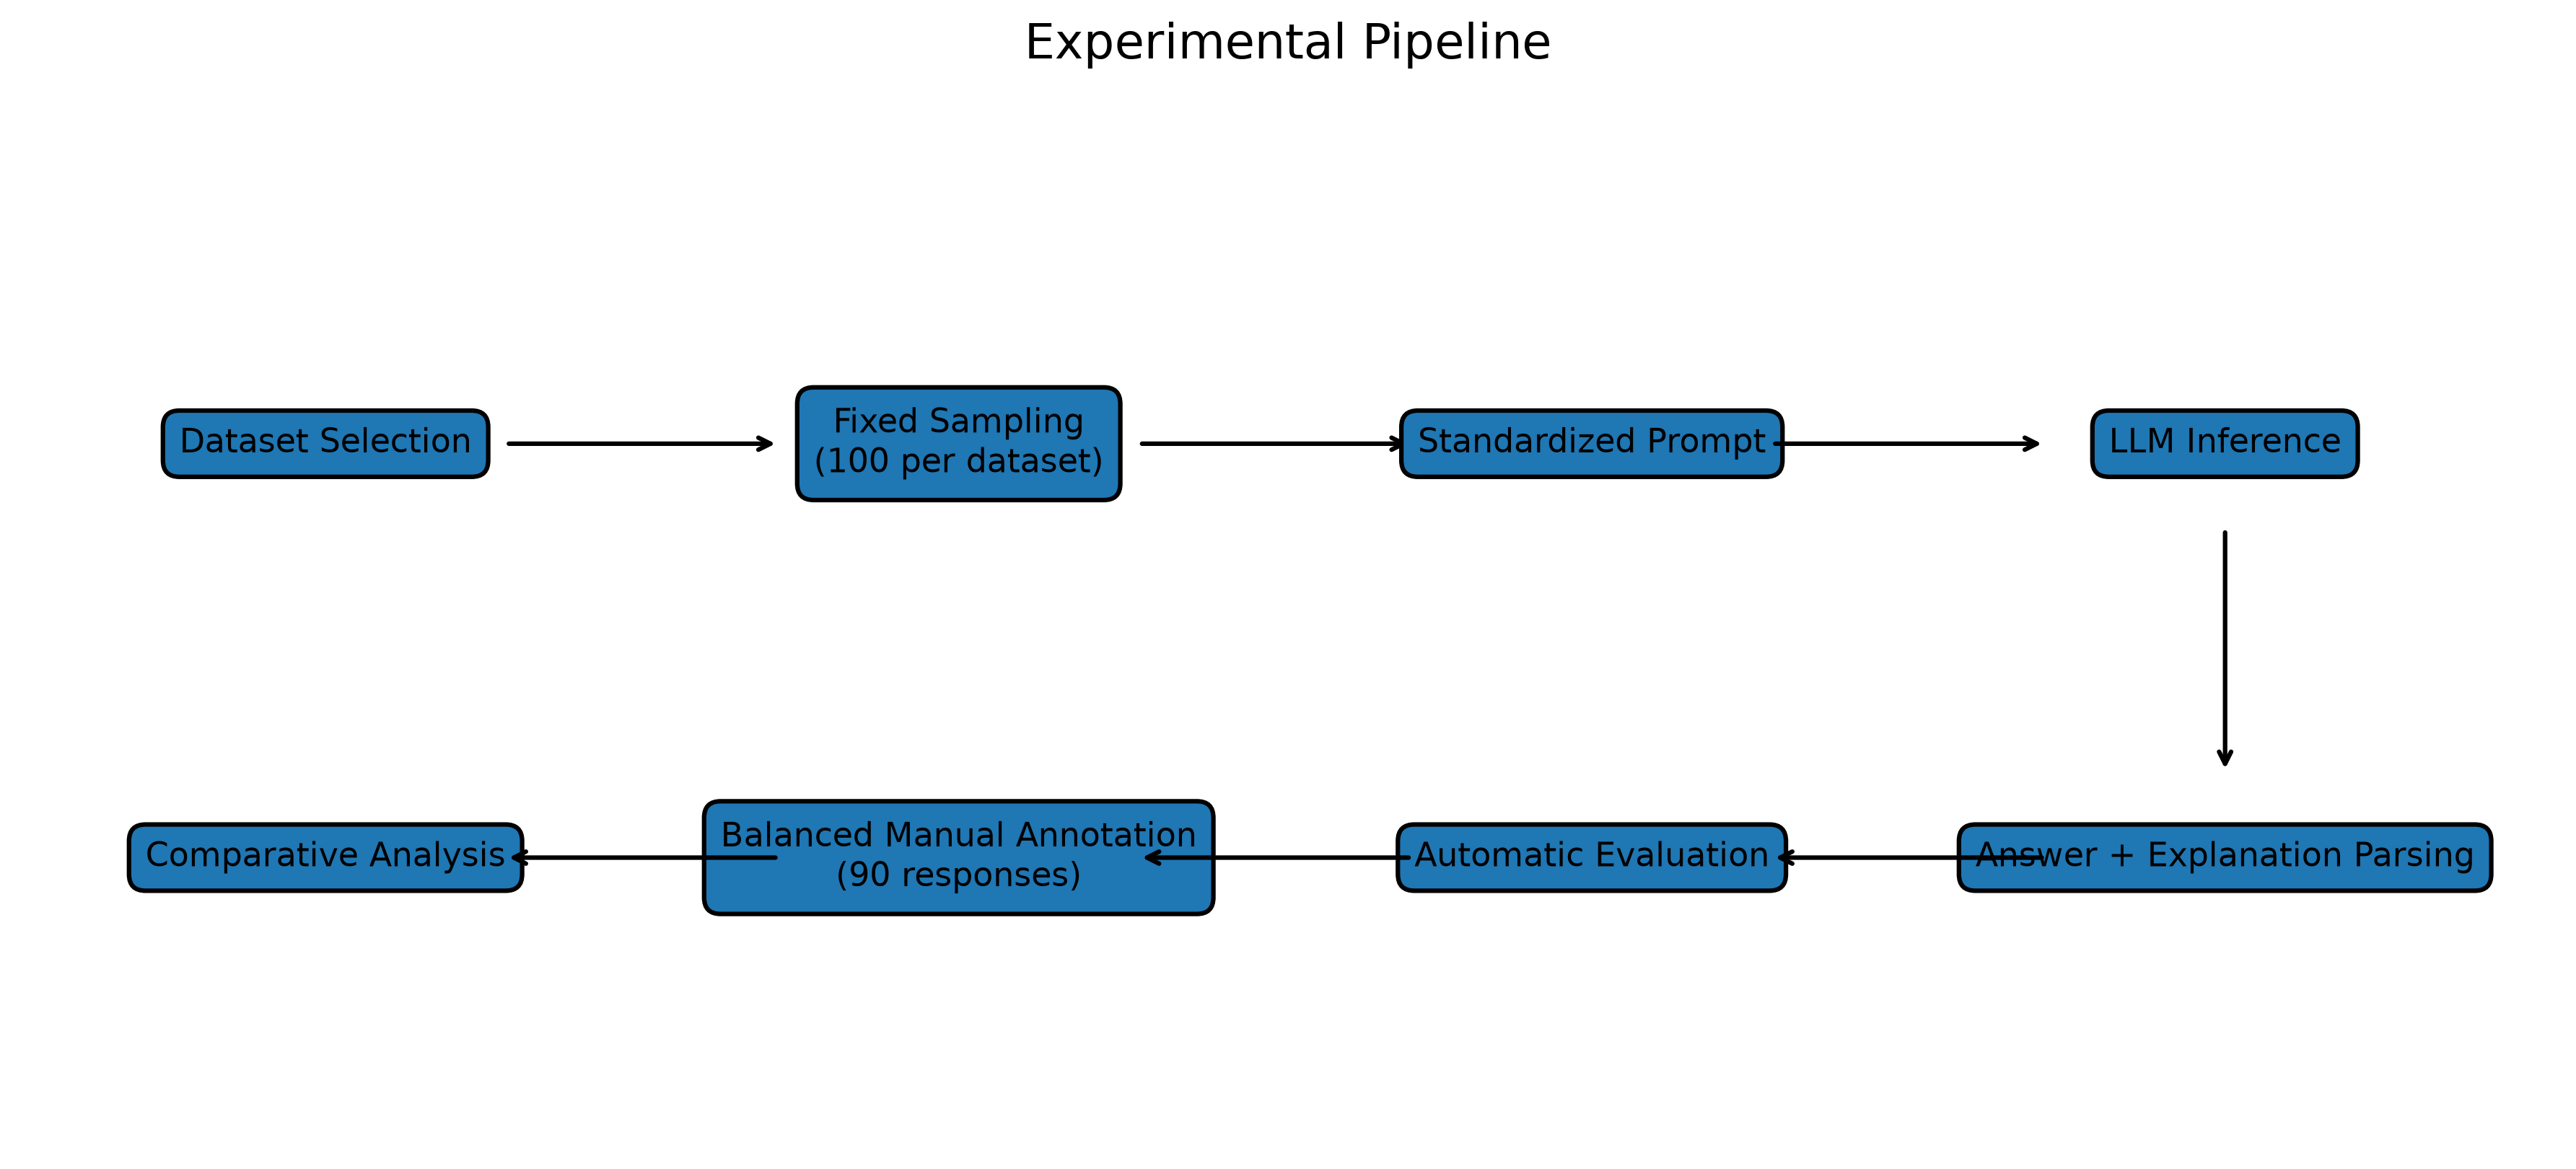
\includegraphics[width=\linewidth]{experimental_pipeline.png}
    \caption{Experimental pipeline. Each model was evaluated on 100
    fixed samples from each dataset, followed by automatic answer
    evaluation and balanced manual annotation of 90 explanations.}
    \label{fig:pipeline}
\end{figure}

The design separates four evaluation dimensions: predictive
performance, instruction compliance, computational efficiency, and
explanation quality. This separation is important because a model may
achieve high answer accuracy while producing outputs that are difficult
to parse, may generate concise but incomplete explanations, or may
produce an explanation that appears coherent while supporting an
incorrect final answer.

\subsection{Research Questions and Operationalization}

RQ1 is operationalized through answer accuracy for each
model--dataset pair and through overall accuracy across all 300
questions per model. Wilson 95\% confidence intervals are reported to
quantify uncertainty around the observed accuracy values.

RQ2 is evaluated using strict parse success, defined as the presence
of both required output fields in the prescribed structure. Mean
generation time is additionally reported to characterize the
efficiency cost of producing the required response.

RQ3 is evaluated using reviewed manual scores from 0 to 3 for
explanation-support faithfulness, logical consistency, and
completeness. The manually analyzed sample contains equal numbers of
correct and incorrect responses within every model--dataset
combination. Faithfulness scores for correct and incorrect answers are
compared using a two-sided Mann--Whitney U test, Cliff's delta, and a
bootstrap 95\% confidence interval for the mean difference.

RQ4 is examined through a primary failure taxonomy applied to the
manually reviewed subset. The categories include answer--explanation
mismatch, arithmetic error, contradictory explanation, factual
hallucination, incomplete reasoning, instruction-following failure,
logical error, unsupported justification, other, and no primary
failure.

\subsection{Selected Models}

Table~\ref{tab:models} summarizes the evaluated models. The selection
contains two general-purpose instruction-tuned models of approximately
3B parameters and one smaller reasoning-distilled model. This design
enables comparison between broadly capable instruction-following
models and a model optimized more explicitly for reasoning-oriented
generation.

\begin{table}[t]
\centering
\small
\caption{Evaluated language models. All models were loaded using
4-bit NF4 quantization.}
\label{tab:models}
\begin{tabular}{p{3.0cm}p{5.7cm}p{1.7cm}}
\toprule
\textbf{Model} &
\textbf{Hugging Face identifier} &
\textbf{Precision} \\
\midrule
Qwen 2.5 3B &
\texttt{Qwen/Qwen2.5-3B-Instruct} &
4-bit NF4 \\

Llama 3.2 3B &
\texttt{meta-llama/Llama-3.2-3B-Instruct} &
4-bit NF4 \\

DeepSeek-R1 Distill 1.5B &
\texttt{deepseek-ai/DeepSeek-R1-Distill-Qwen-1.5B} &
4-bit NF4 \\
\bottomrule
\end{tabular}
\end{table}

Qwen~2.5 is a multilingual instruction-tuned model family designed
for a broad range of language and reasoning tasks
\cite{qwen2024qwen25}. Llama~3.2~3B is a compact open-weight
instruction model from the Llama family
\cite{grattafiori2024llama3}. DeepSeek-R1 Distill Qwen~1.5B is a
reasoning-oriented distilled model derived from DeepSeek-R1
\cite{deepseek2025r1}. All models were loaded using 4-bit NF4
quantization because the experiments were conducted on a consumer GPU
with 4\,GB of video memory.

\subsection{Reasoning Datasets}

The benchmark contains three datasets representing complementary
reasoning requirements:

\begin{itemize}
    \item \textbf{GSM8K} contains grade-school mathematical word
    problems that require arithmetic and multi-step numerical
    reasoning \cite{cobbe2021gsm8k}.

    \item \textbf{CommonsenseQA} contains five-option
    multiple-choice questions requiring ordinary world knowledge,
    semantic associations, and commonsense reasoning
    \cite{talmor2019commonsenseqa}.

    \item \textbf{StrategyQA} contains binary yes/no questions whose
    answers often require implicit decomposition and the combination
    of multiple supporting facts \cite{geva2021strategyqa}.
\end{itemize}

Exactly 100 examples were sampled from each dataset using random seed
42. GSM8K examples were drawn from the test split, CommonsenseQA
examples from the validation split, and StrategyQA examples from the
available training split of a Parquet-compatible distribution. The
resulting benchmark contained 300 unique questions and was frozen
before the final inference runs. The processed CSV and JSONL benchmark
files were checksummed to support reproducibility. The checksum and
data-preparation commands are reported in the appendix.

\subsection{Prompt Design}

Every model received the same standardized instruction and was required
to return exactly two fields:

\begin{quote}
\texttt{FINAL\_ANSWER: <answer>}\\
\texttt{EXPLANATION: <concise justification>}
\end{quote}

For GSM8K, the final answer was expected to be a numerical value or a
short numerical expression. For CommonsenseQA, the required answer was
the selected option label, with option text permitted as additional
content. For StrategyQA, the answer was normalized to a binary
yes/no representation.

The answer was requested before the explanation to make the final
prediction easy to identify and parse. The explanation was explicitly
constrained to be concise. Using the same prompt structure for all
models reduced model-specific prompt engineering and enabled a common
parsing and evaluation procedure.

\subsection{Evaluation Protocol}

Inference was conducted separately for every model--dataset
combination. Generated outputs were written incrementally to JSONL
files so that interrupted runs could resume without regenerating
completed samples. After generation, a strict parser attempted to
extract the required \texttt{FINAL\_ANSWER} and
\texttt{EXPLANATION} fields.

The extracted answers were normalized using dataset-specific rules and
compared with the corresponding ground-truth labels. The scored outputs
were subsequently merged into model-level and cross-model result
tables.

The complete experiment produced 900 responses:

\[
3\ \text{models}
\times
3\ \text{datasets}
\times
100\ \text{samples}
=
900\ \text{responses}.
\]

\subsection{Automatic Evaluation Metrics}

Automatic evaluation measured four properties:

\begin{itemize}
    \item \textbf{Answer accuracy}: the proportion of responses whose
    normalized final answer matched the dataset ground truth.

    \item \textbf{Strict parse success}: whether the model produced
    both required fields in the prescribed answer--explanation
    structure.

    \item \textbf{Generation time}: the elapsed inference time for
    producing each response.

    \item \textbf{Explanation length}: the number of whitespace-
    separated words in the extracted explanation.
\end{itemize}

For GSM8K, numerical answers were normalized before comparison.
CommonsenseQA outputs were evaluated primarily through their option
labels. StrategyQA outputs were mapped across equivalent
representations, including \texttt{A/B}, \texttt{yes/no}, and
\texttt{true/false}.

Strict parse success was retained as a separate measure rather than
silently repairing every malformed response. This decision treats
output-format compliance as an important aspect of practical
instruction following.

\subsection{Manual Explanation Analysis}

A balanced subset of 90 successfully parsed responses was selected for
manual explanation analysis. The sample contained 10 responses from
every model--dataset combination. Within each combination, five correct
and five incorrect answers were selected whenever possible. Each model
therefore contributed 30 reviewed responses.

The selected explanations were evaluated on three dimensions:

\begin{itemize}
    \item \textbf{Explanation-support faithfulness}: whether the
    explanation correctly supports the model's stated final answer;

    \item \textbf{Logical consistency}: whether the reasoning is
    internally coherent and free from contradiction;

    \item \textbf{Completeness}: whether the explanation contains
    sufficient reasoning to justify the stated answer.
\end{itemize}

Each dimension was assigned a score from 0 to 3 according to
Table~\ref{tab:rubric}.

\begin{table}[t]
\centering
\caption{Manual explanation-scoring rubric.}
\label{tab:rubric}
\begin{tabular}{cp{8.2cm}}
\toprule
\textbf{Score} & \textbf{Interpretation} \\
\midrule
0 &
The explanation is contradictory, unrelated, absent, or provides no
meaningful support. \\

1 &
The explanation contains major errors or provides only very weak
support for the stated answer. \\

2 &
The explanation provides partial support but contains missing,
unsupported, or flawed reasoning. \\

3 &
The explanation provides clear, correct, consistent, and sufficient
support for the stated answer. \\
\bottomrule
\end{tabular}
\end{table}

A primary failure category was additionally assigned to each response.
The taxonomy contained:

\begin{itemize}
    \item answer--explanation mismatch;
    \item arithmetic error;
    \item contradictory explanation;
    \item factual hallucination;
    \item incomplete reasoning;
    \item instruction-following failure;
    \item logical error;
    \item unsupported justification;
    \item other;
    \item no primary failure.
\end{itemize}

The annotations evaluate visible behavioral support. They do not
establish that the textual explanation is causally identical to the
hidden computation responsible for the model's prediction. This
distinction follows previous warnings against interpreting generated
rationales as direct access to internal model reasoning
\cite{turpin2023language,lanham2023measuring}.

\subsection{Statistical Analysis}

Wilson 95\% confidence intervals were calculated for answer accuracy
at both the dataset and overall model levels. Wilson intervals were
chosen because accuracy is a binomial proportion and each
model--dataset estimate was based on 100 observations.

Because the manual explanation scores are ordinal values on a 0--3
scale, the faithfulness distributions for correct and incorrect answers
were compared using a two-sided Mann--Whitney U test. Cliff's delta was
used as a non-parametric effect-size measure. Positive values indicate
that explanations attached to correct answers tend to receive higher
faithfulness scores.

A non-parametric bootstrap with 10,000 resamples and random seed 42
was additionally used to estimate a 95\% confidence interval for the
difference between the mean faithfulness score of correct and incorrect
answers. Statistical analyses were performed both across all 90
reviewed responses and separately for each model.

\section{Experimental Setup}

The experimental setup was designed to maximize reproducibility within
the constraints of local consumer hardware. Model configurations,
benchmark samples, prompts, generated responses, parsed outputs,
evaluation scores, and analysis files were stored in a structured,
version-controlled project.

\subsection{Hardware and Software}

Experiments were conducted on a Windows system using Python~3.11.2,
PyTorch~2.7.1 with CUDA~11.8, and an NVIDIA GeForce GTX~1650~Ti
with 4\,GB of VRAM. Hugging Face Transformers and Datasets were used
for model inference and dataset processing. bitsandbytes and Accelerate
were used for quantized model loading and device placement. Pandas,
SciPy, NumPy, and Matplotlib were used for evaluation, statistical
analysis, and visualization.

\subsection{Model Configuration}

All models were loaded through their official Hugging Face
configurations and chat templates. Automatic device placement was used.
Where required, the tokenizer padding token was mapped to the
end-of-sequence token.

Quantized loading used 4-bit NF4 weights with double quantization and
float16 computation. The same quantization configuration was applied
to all three models to fit them within the available 4\,GB GPU memory.

\subsection{Generation Settings}

Greedy deterministic decoding was used to improve reproducibility.
Sampling was disabled and the random seed was fixed to 42. Qwen and
Llama used a maximum generation budget of 256 new tokens.

DeepSeek initially produced a high proportion of truncated or
incomplete responses under the same 256-token limit because of its
longer reasoning traces. Its final evaluation therefore used a maximum
of 768 new tokens. This difference is reported explicitly because it
affects generation time, output length, and strict-format success, and
limits direct efficiency comparisons between DeepSeek and the other
models.

\begin{table}[t]
\centering
\caption{Generation configuration used in the final experiments.}
\label{tab:generation}
\begin{tabular}{ll}
\toprule
\textbf{Parameter} & \textbf{Value} \\
\midrule
Decoding strategy & Greedy \\
Sampling & Disabled \\
Random seed & 42 \\
Qwen maximum new tokens & 256 \\
Llama maximum new tokens & 256 \\
DeepSeek maximum new tokens & 768 \\
Quantization & 4-bit NF4 \\
Double quantization & Enabled \\
Computation type & Float16 \\
\bottomrule
\end{tabular}
\end{table}

\subsection{Experimental Procedure}

For each model, a pilot response was first generated to verify model
loading, prompt formatting, output parsing, and result storage. The
final evaluation then generated 100 responses for each dataset. Because
greedy decoding was used with fixed settings, repeated inference under
the same configuration was deterministic.

Generated outputs were scored separately for each dataset and then
combined into a 900-row master results file. Each row preserved the
sample identifier, model identifier, dataset, prompt, raw generation,
parsed final answer, extracted explanation, timing information, parse
status, correctness label, and error field.

DeepSeek initially used the same 256-token generation limit as Qwen and
Llama. However, many outputs were truncated before the required
\texttt{FINAL\_ANSWER} and \texttt{EXPLANATION} fields were completed.
Inspection of the raw generations showed that the model was still
producing long reasoning traces when generation stopped. The final
DeepSeek run therefore used a maximum of 768 new tokens. This larger
budget improved completion and parse success but also increased runtime
and limits direct efficiency comparison with the other models.

\subsection{Reproducibility}

The final benchmark was generated using random seed 42 and stored in
both CSV and JSONL formats. A SHA-256 checksum was recorded after the
StrategyQA samples were added. The final outputs preserve all
intermediate information required to reproduce the evaluation,
including model and sample identifiers, raw generations, parsed fields,
timing information, correctness labels, parse status, and error
messages.

The code, configuration files, processed benchmark, evaluation scripts,
manual-analysis files, statistical outputs, and paper figures are
maintained in the FaithfulLLM project repository. The final benchmark
checksum and reproduction commands are provided in the appendix.

\section{Results}

\subsection{Answer Accuracy}

Table~\ref{tab:accuracy} summarizes answer accuracy for all
model--dataset combinations. Figure~\ref{fig:accuracy_ci} presents the
same results with 95\% Wilson confidence intervals.

\begin{table}[t]
\centering
\caption{Answer accuracy (\%) by model and dataset.}
\label{tab:accuracy}
\begin{tabular}{lrrrr}
\toprule
\textbf{Model} &
\textbf{GSM8K} &
\textbf{CSQA} &
\textbf{StrategyQA} &
\textbf{Overall} \\
\midrule
Qwen 2.5 3B & 13 & 76 & 60 & 49.67 \\
Llama 3.2 3B & 6 & 70 & 59 & 45.00 \\
DeepSeek-R1 Distill 1.5B & 80 & 28 & 49 & 52.33 \\
\bottomrule
\end{tabular}
\end{table}

\begin{figure}[t]
    \centering
    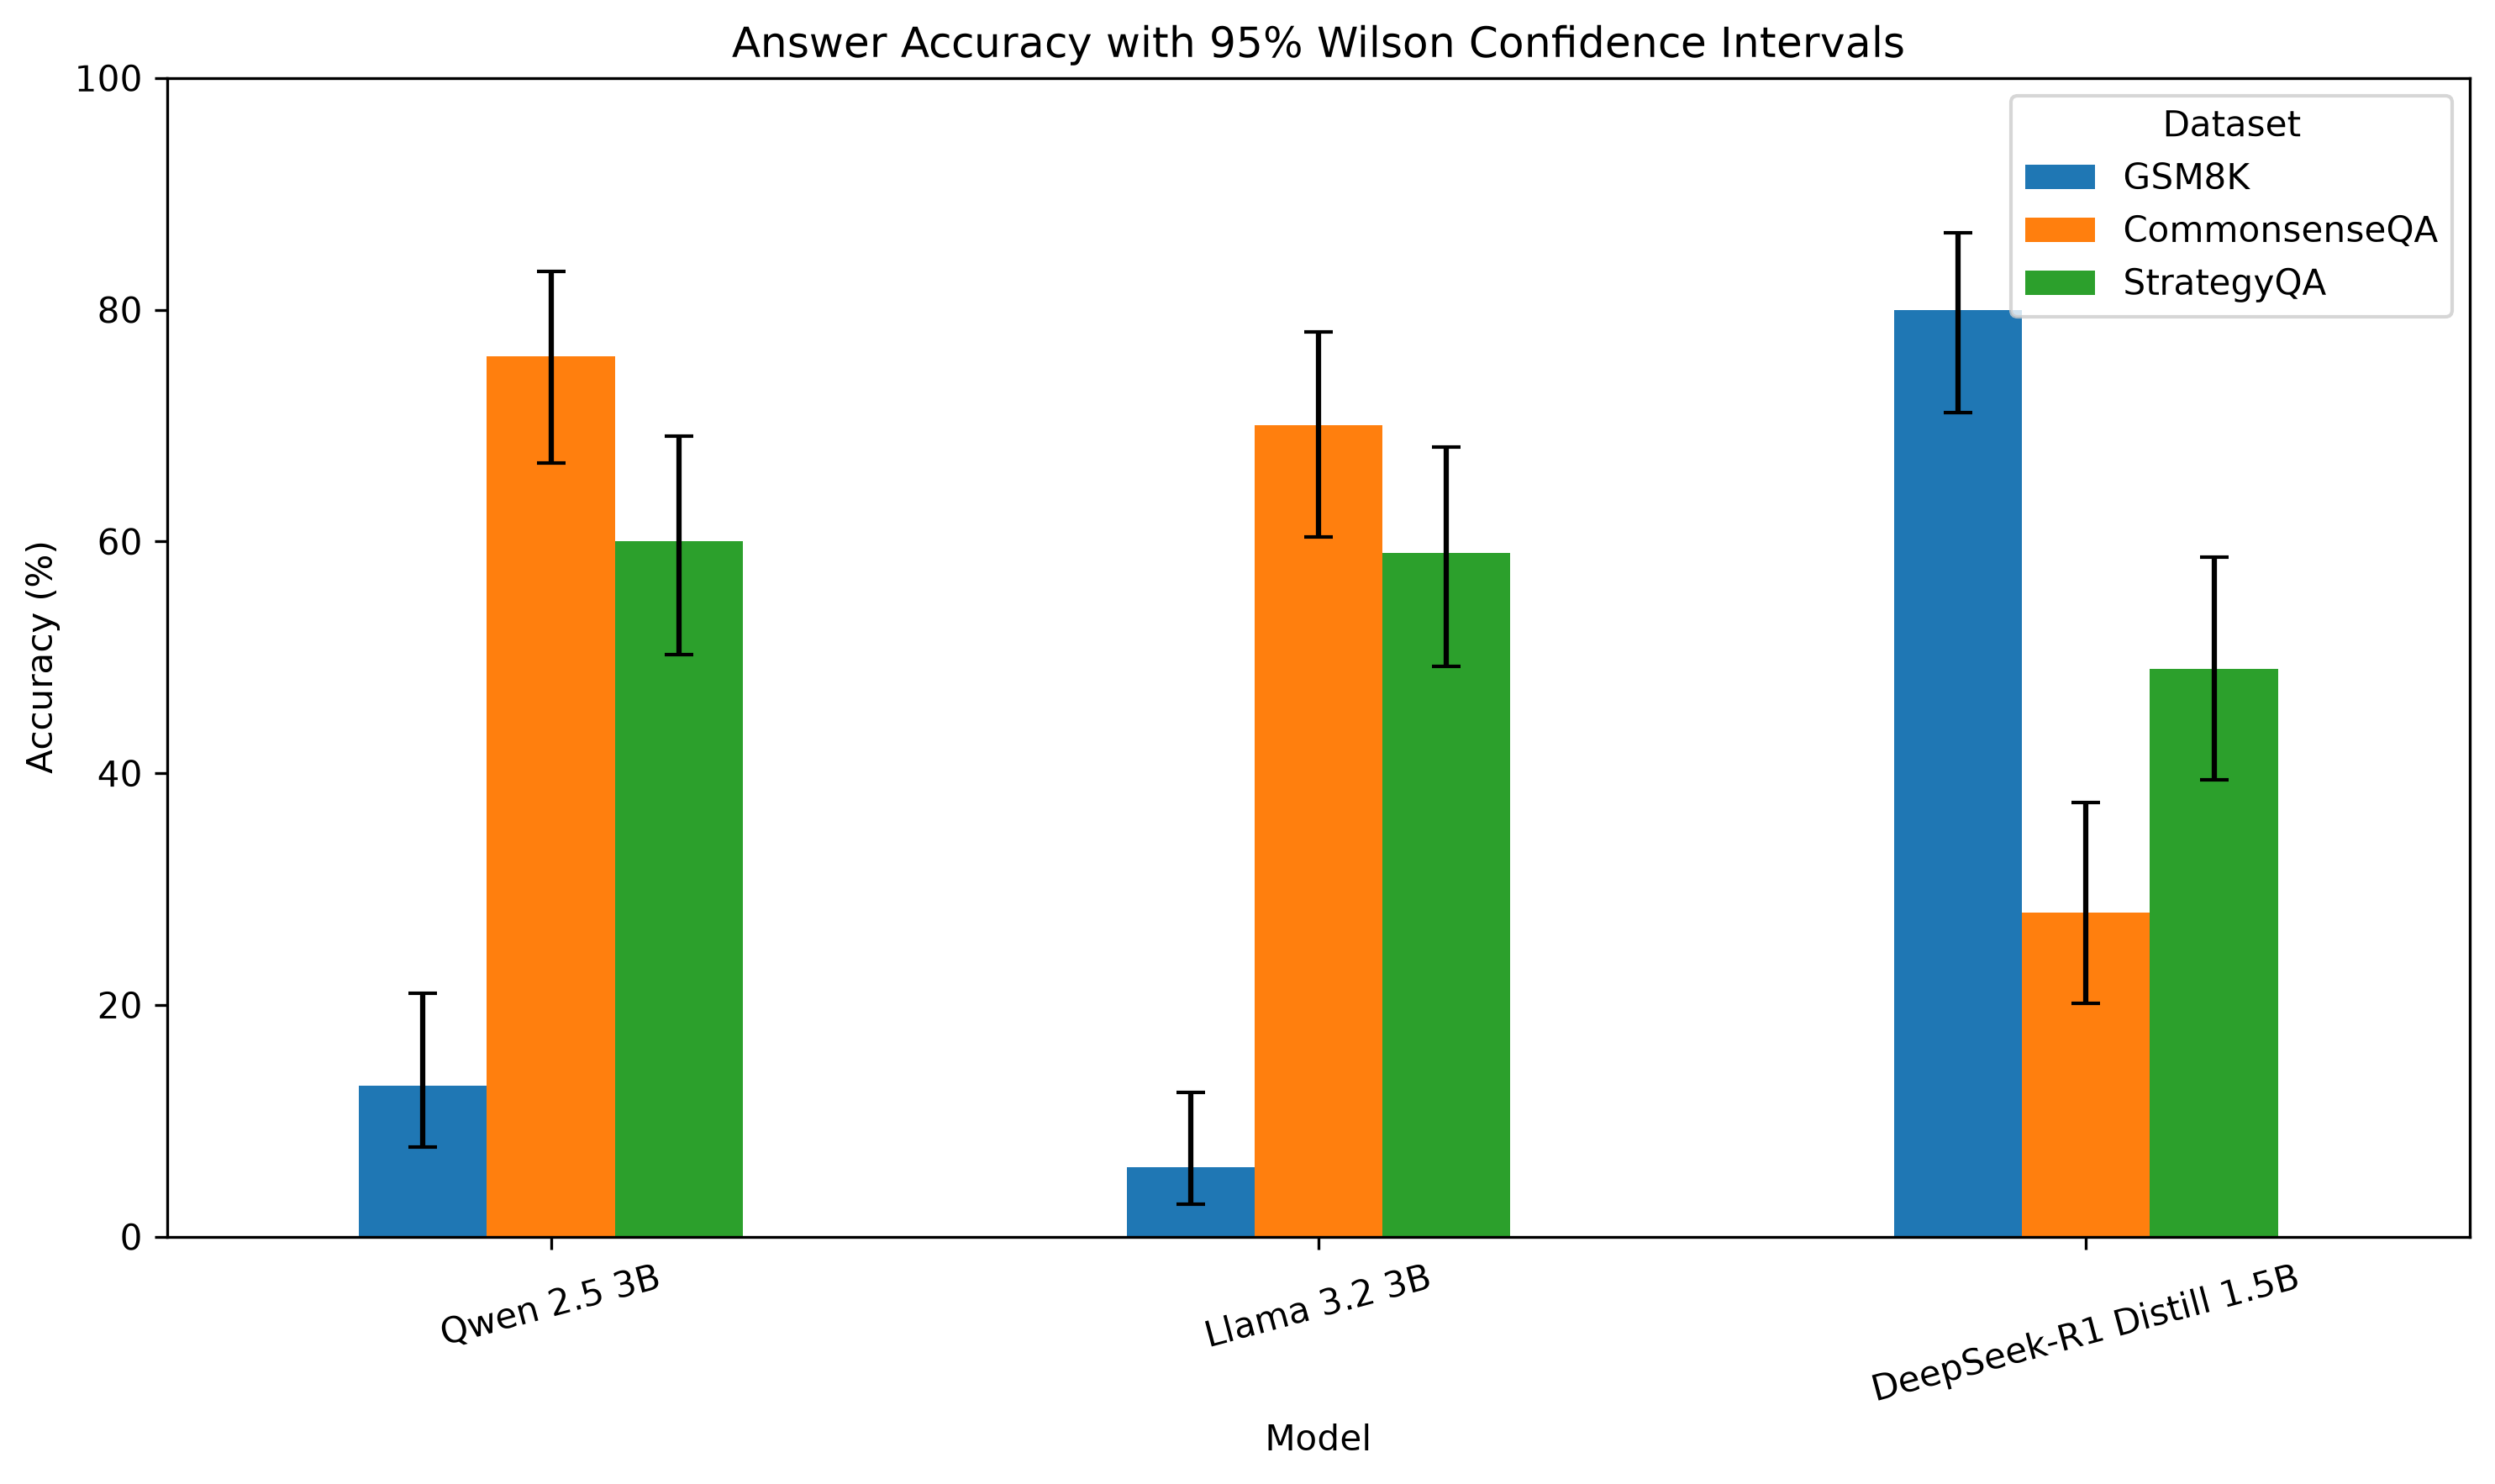
\includegraphics[width=\linewidth]
    {accuracy_with_confidence_intervals.png}
    \caption{Answer accuracy by model and dataset with 95\% Wilson
    confidence intervals. Each estimate is based on 100 samples.}
    \label{fig:accuracy_ci}
\end{figure}

The results reveal strong task specialization. DeepSeek-R1 Distill
achieved 80.00\% accuracy on GSM8K
(95\% CI: 71.12--86.66), far above Qwen at 13.00\%
(95\% CI: 7.76--20.98) and Llama at 6.00\%
(95\% CI: 2.78--12.48).

In contrast, Qwen achieved the highest observed CommonsenseQA accuracy
at 76.00\% (95\% CI: 66.77--83.31) and the highest observed StrategyQA
accuracy at 60.00\% (95\% CI: 50.20--69.06). Llama followed closely on
CommonsenseQA at 70.00\% and StrategyQA at 59.00\%.

At the overall level, DeepSeek achieved the highest observed accuracy
at 52.33\% (95\% CI: 46.69--57.92), followed by Qwen at 49.67\%
(95\% CI: 44.05--55.29) and Llama at 45.00\%
(95\% CI: 39.47--50.66). Because the overall confidence intervals
overlap substantially, these values should not be interpreted as
decisive evidence that one model is universally superior.

\subsection{Format Compliance and Runtime}

Table~\ref{tab:efficiency} reports strict parse success and mean
generation time. Llama followed the required output structure for all
300 responses. Qwen failed to produce both required fields in only two
responses. DeepSeek obtained the lowest strict parse success because
several outputs contained long reasoning loops, incomplete generations,
or a final answer without the required explanation field.

\begin{table}[t]
\centering
\caption{Overall strict parse success and mean generation time.}
\label{tab:efficiency}
\begin{tabular}{lrr}
\toprule
\textbf{Model} &
\textbf{Parse success (\%)} &
\textbf{Mean time (s)} \\
\midrule
Qwen 2.5 3B & 99.33 & 10.21 \\
Llama 3.2 3B & 100.00 & 7.57 \\
DeepSeek-R1 Distill 1.5B & 85.67 & 37.01 \\
\bottomrule
\end{tabular}
\end{table}

DeepSeek was substantially slower than Qwen and Llama. This difference
is consistent with its longer reasoning traces and larger generation
budget. Its strong GSM8K performance therefore came with a practical
cost in inference time and output-format reliability. Because DeepSeek
used 768 maximum new tokens while the other models used 256, the runtime
comparison should be interpreted as a practical system-level comparison
rather than a strictly controlled token-budget comparison.

\subsection{Manual Explanation Scores}

Table~\ref{tab:manual_scores} summarizes mean manual scores across 30
reviewed responses per model.

\begin{table}[t]
\centering
\caption{Mean reviewed explanation scores on a 0--3 scale.}
\label{tab:manual_scores}
\begin{tabular}{lrrr}
\toprule
\textbf{Model} &
\textbf{Faithfulness} &
\textbf{Logic} &
\textbf{Completeness} \\
\midrule
DeepSeek-R1 Distill 1.5B & 1.87 & 2.07 & 2.03 \\
Llama 3.2 3B & 1.70 & 2.20 & 2.17 \\
Qwen 2.5 3B & 1.73 & 2.13 & 2.30 \\
\bottomrule
\end{tabular}
\end{table}

DeepSeek obtained the highest mean explanation-support faithfulness
score. Llama achieved the highest mean logical-consistency score, while
Qwen achieved the highest mean completeness score. The differences are
moderate and do not support the conclusion that one model is uniformly
best across all explanation dimensions.

\subsection{Faithfulness by Dataset}

Figure~\ref{fig:faithfulness_heatmap} shows substantial task-dependent
variation in explanation-support faithfulness.

\begin{figure}[t]
    \centering
    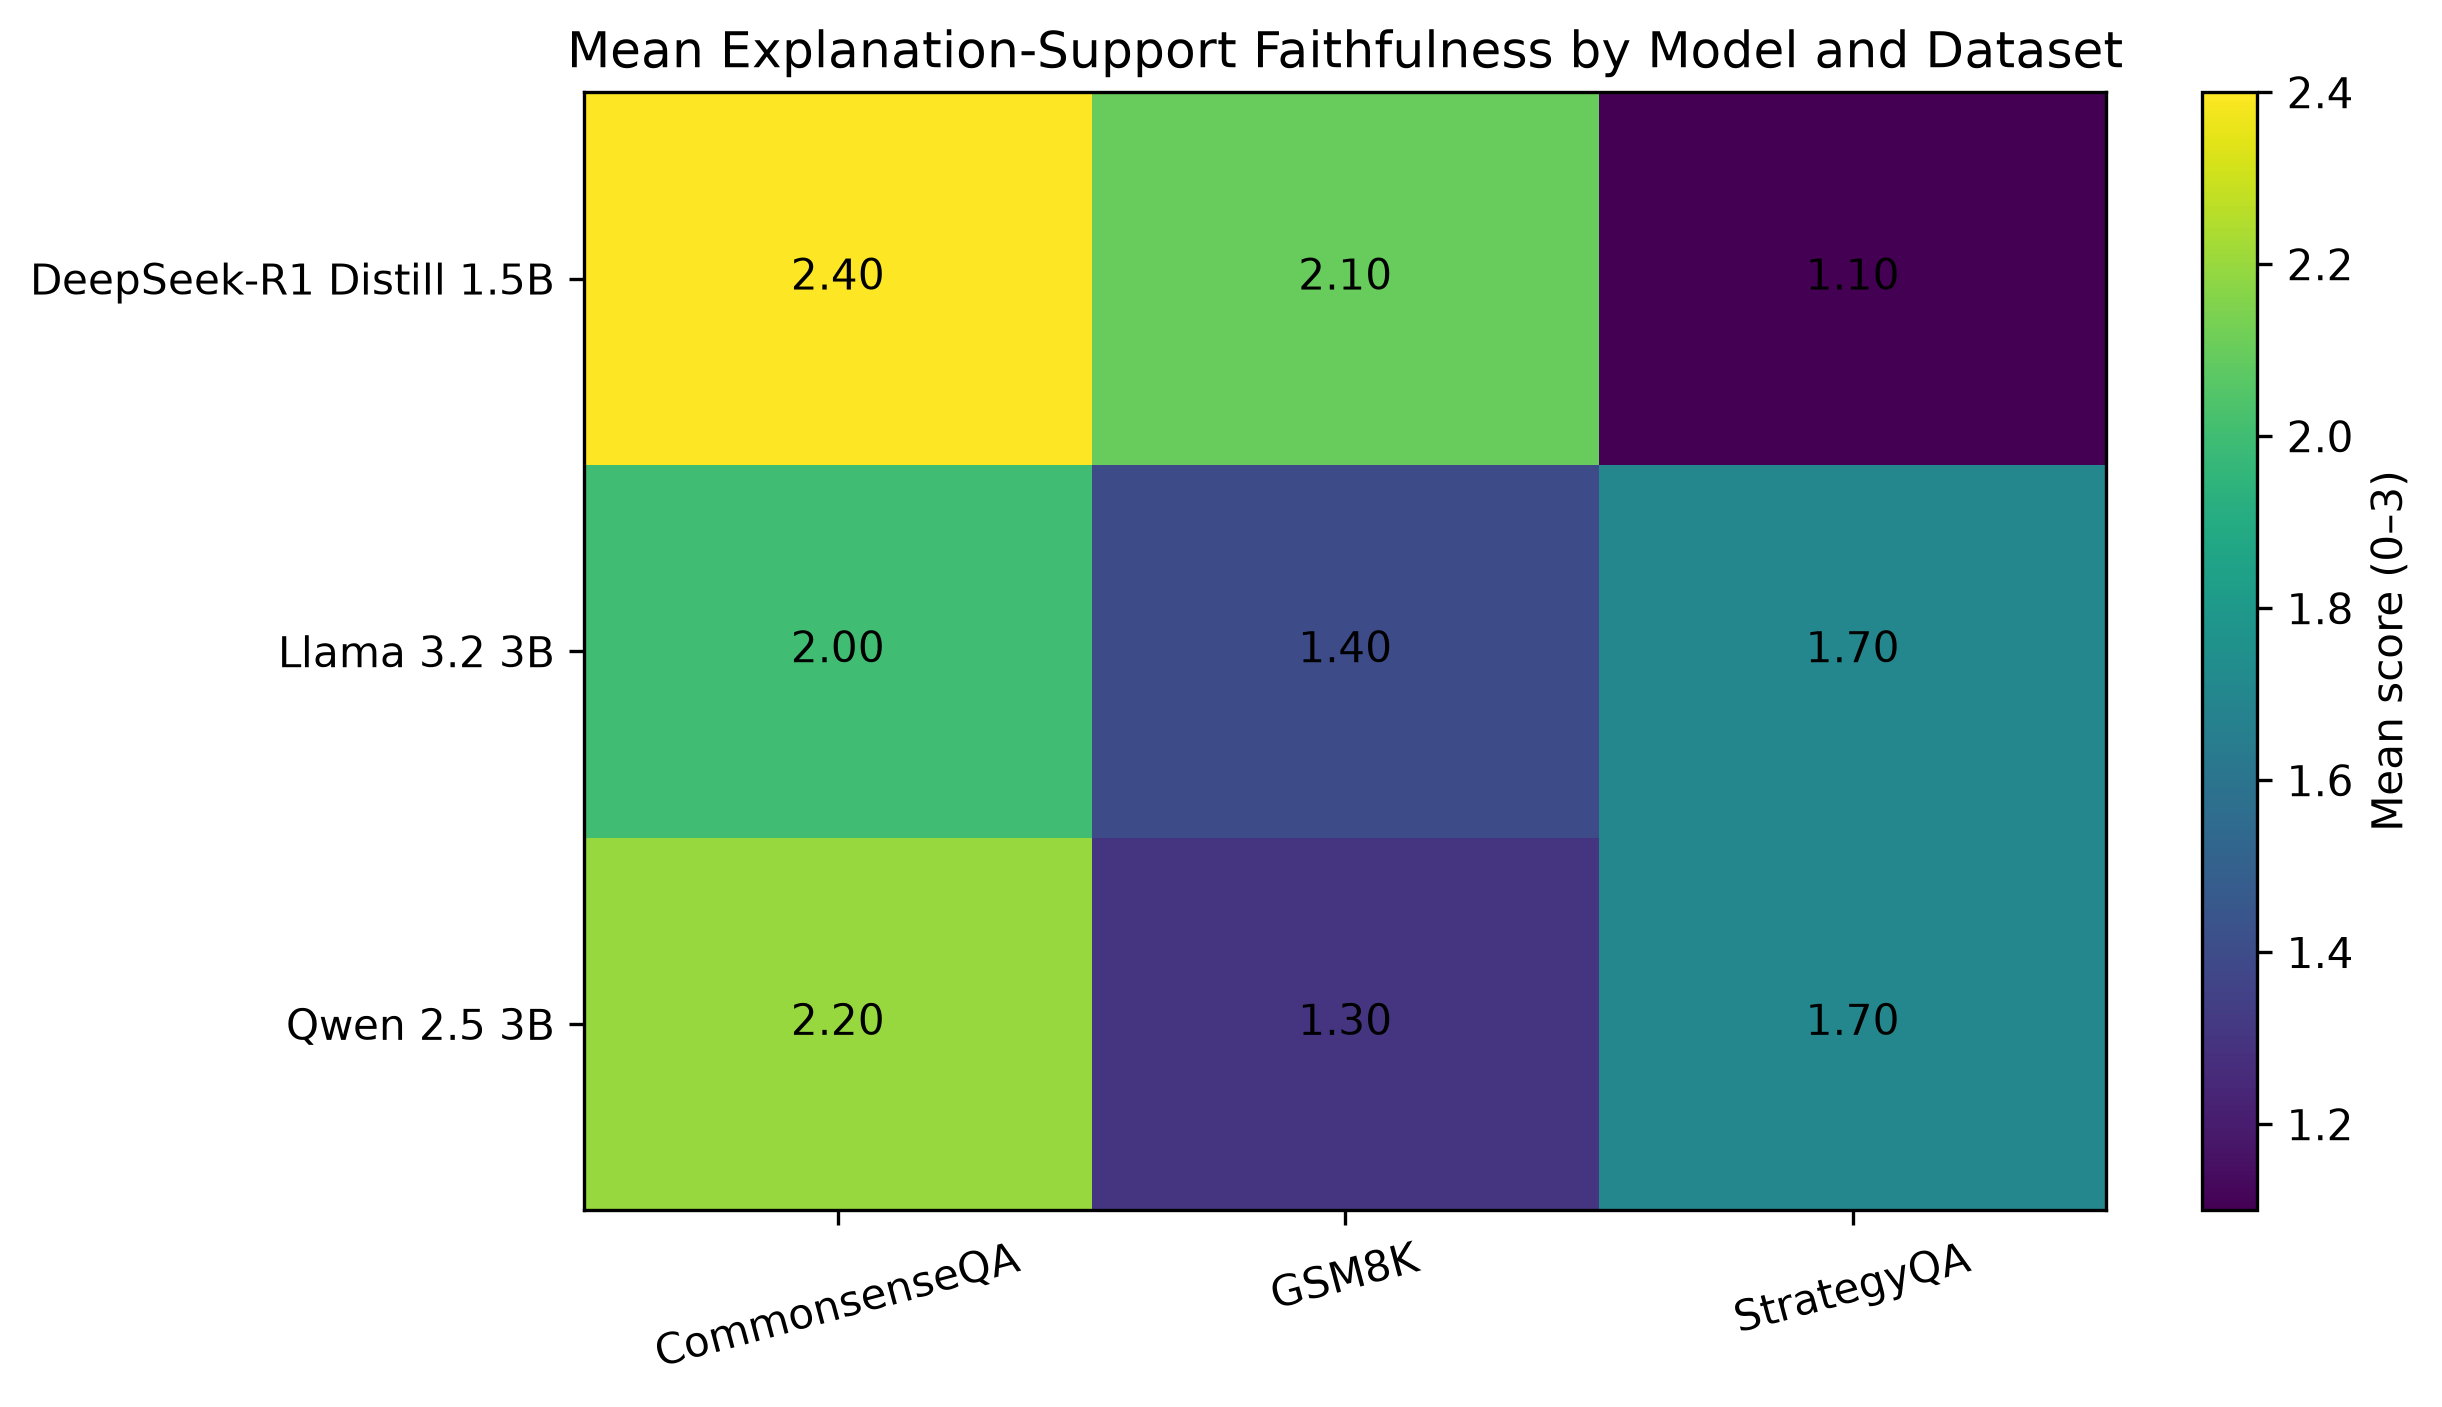
\includegraphics[width=\linewidth]{faithfulness_heatmap.png}
    \caption{Mean explanation-support faithfulness score by model and
    dataset. The values show strong task-dependent variation in visible
    explanation quality.}
    \label{fig:faithfulness_heatmap}
\end{figure}

DeepSeek achieved the highest mean faithfulness on CommonsenseQA
(2.40) and GSM8K (2.10), but the lowest score on StrategyQA (1.10).
Llama and Qwen both achieved 1.70 on StrategyQA, while their GSM8K
explanations scored 1.40 and 1.30, respectively. These results reinforce
the finding that explanation quality is strongly task-dependent.

\subsection{Correct vs.\ Incorrect Answers}

Figure~\ref{fig:correct_incorrect} presents the relationship between
answer correctness and explanation-support faithfulness.

\begin{figure}[t]
    \centering
    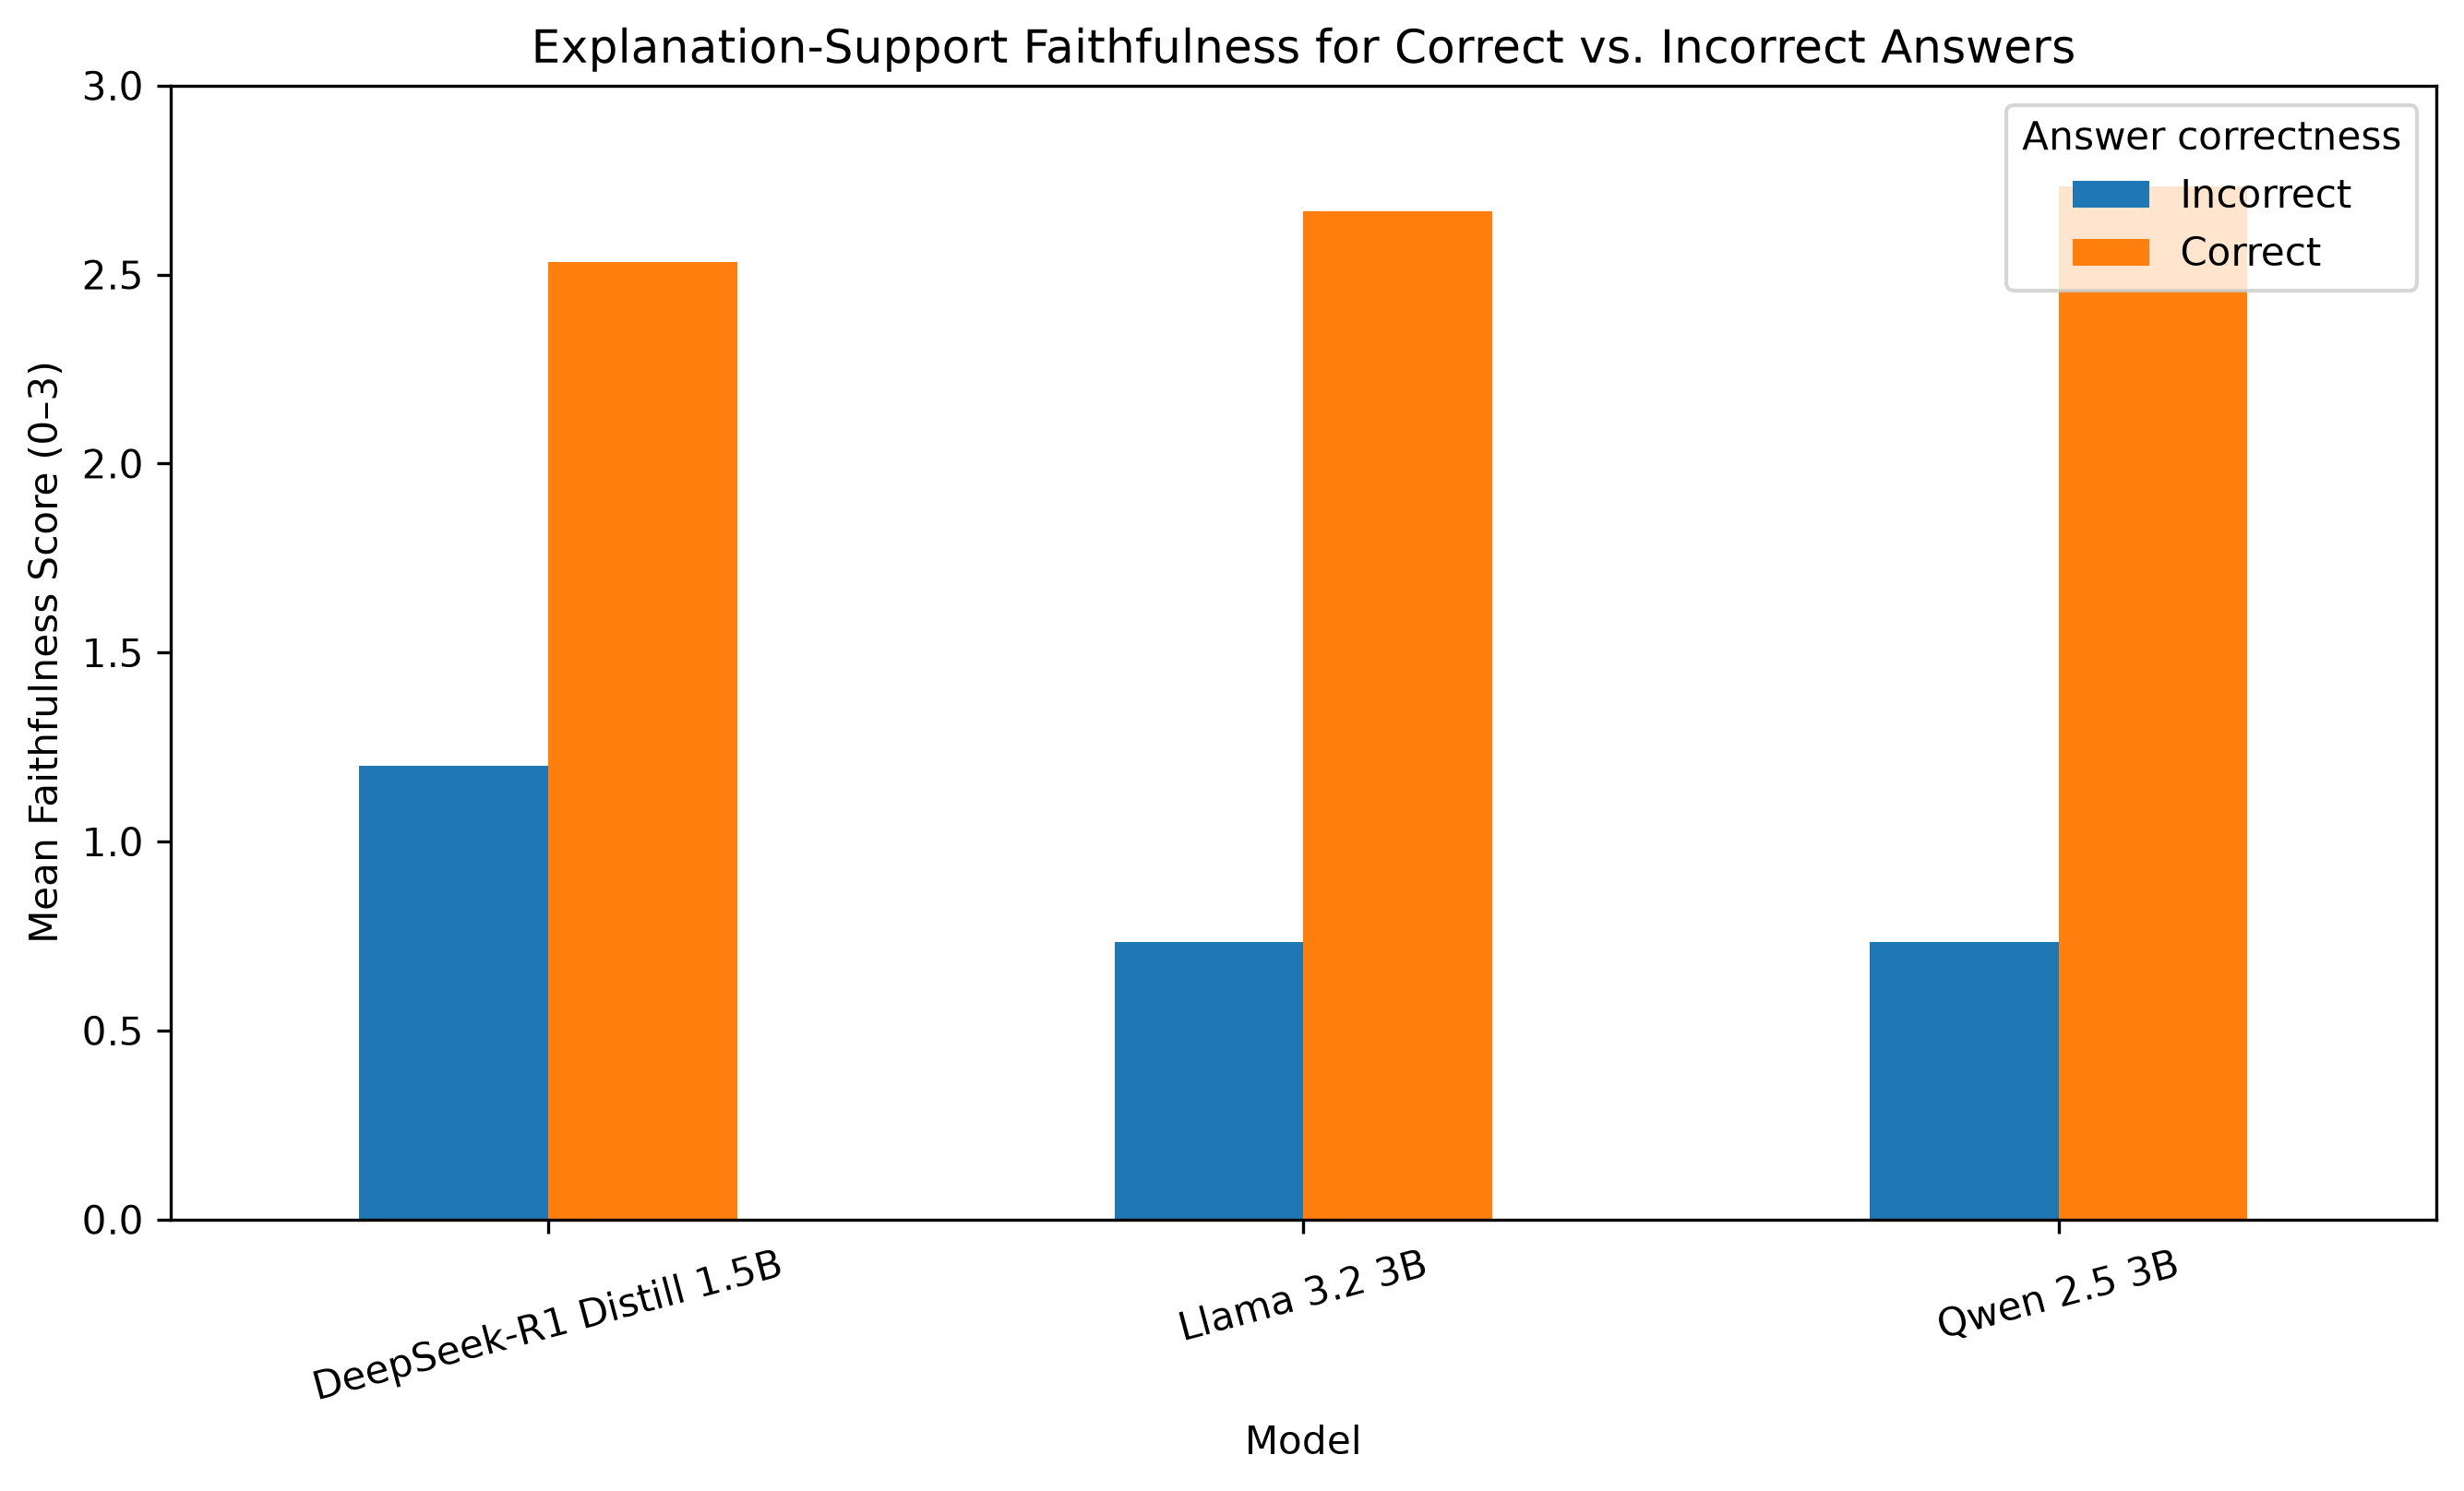
\includegraphics[width=\linewidth]
    {faithfulness_correct_vs_incorrect.png}
    \caption{Mean explanation-support faithfulness scores for correct
    and incorrect answers. Correct answers receive substantially higher
    scores across all evaluated models.}
    \label{fig:correct_incorrect}
\end{figure}

For DeepSeek, the mean score increased from 1.20 for incorrect answers
to 2.53 for correct answers. Llama increased from 0.73 to 2.67, while
Qwen increased from 0.73 to 2.73. These descriptive results indicate a
strong association between answer correctness and visible explanation
quality.

\subsection{Statistical Analysis}

Across all models, explanations accompanying correct answers received a
mean explanation-support faithfulness score of 2.64, compared with 0.89
for explanations accompanying incorrect answers. The mean difference
was 1.76 points, with a bootstrap 95\% confidence interval of
[1.42, 2.07].

A two-sided Mann--Whitney U test showed that the two score
distributions differed significantly
($U=1827.0$, $p<0.001$). Cliff's delta was 0.804, indicating a large
effect.

The effect remained large for every model individually. Qwen showed a
mean difference of 2.00 points
($U=214.0$, $p<0.001$, $\delta=0.902$), while Llama showed a
difference of 1.93 points
($U=211.5$, $p<0.001$, $\delta=0.880$). DeepSeek showed a smaller but
still large difference of 1.33 points
($U=183.0$, $p=0.001$, $\delta=0.627$).

These results support H2 and show that correct answers are strongly
associated with higher visible explanation quality. However, the
analysis does not establish that the explanations causally reflect the
models' hidden internal reasoning processes.

\subsection{Failure Categories}

Figure~\ref{fig:failure_categories} summarizes the primary failure
types in the balanced manual-analysis sample.

\begin{figure}[t]
    \centering
    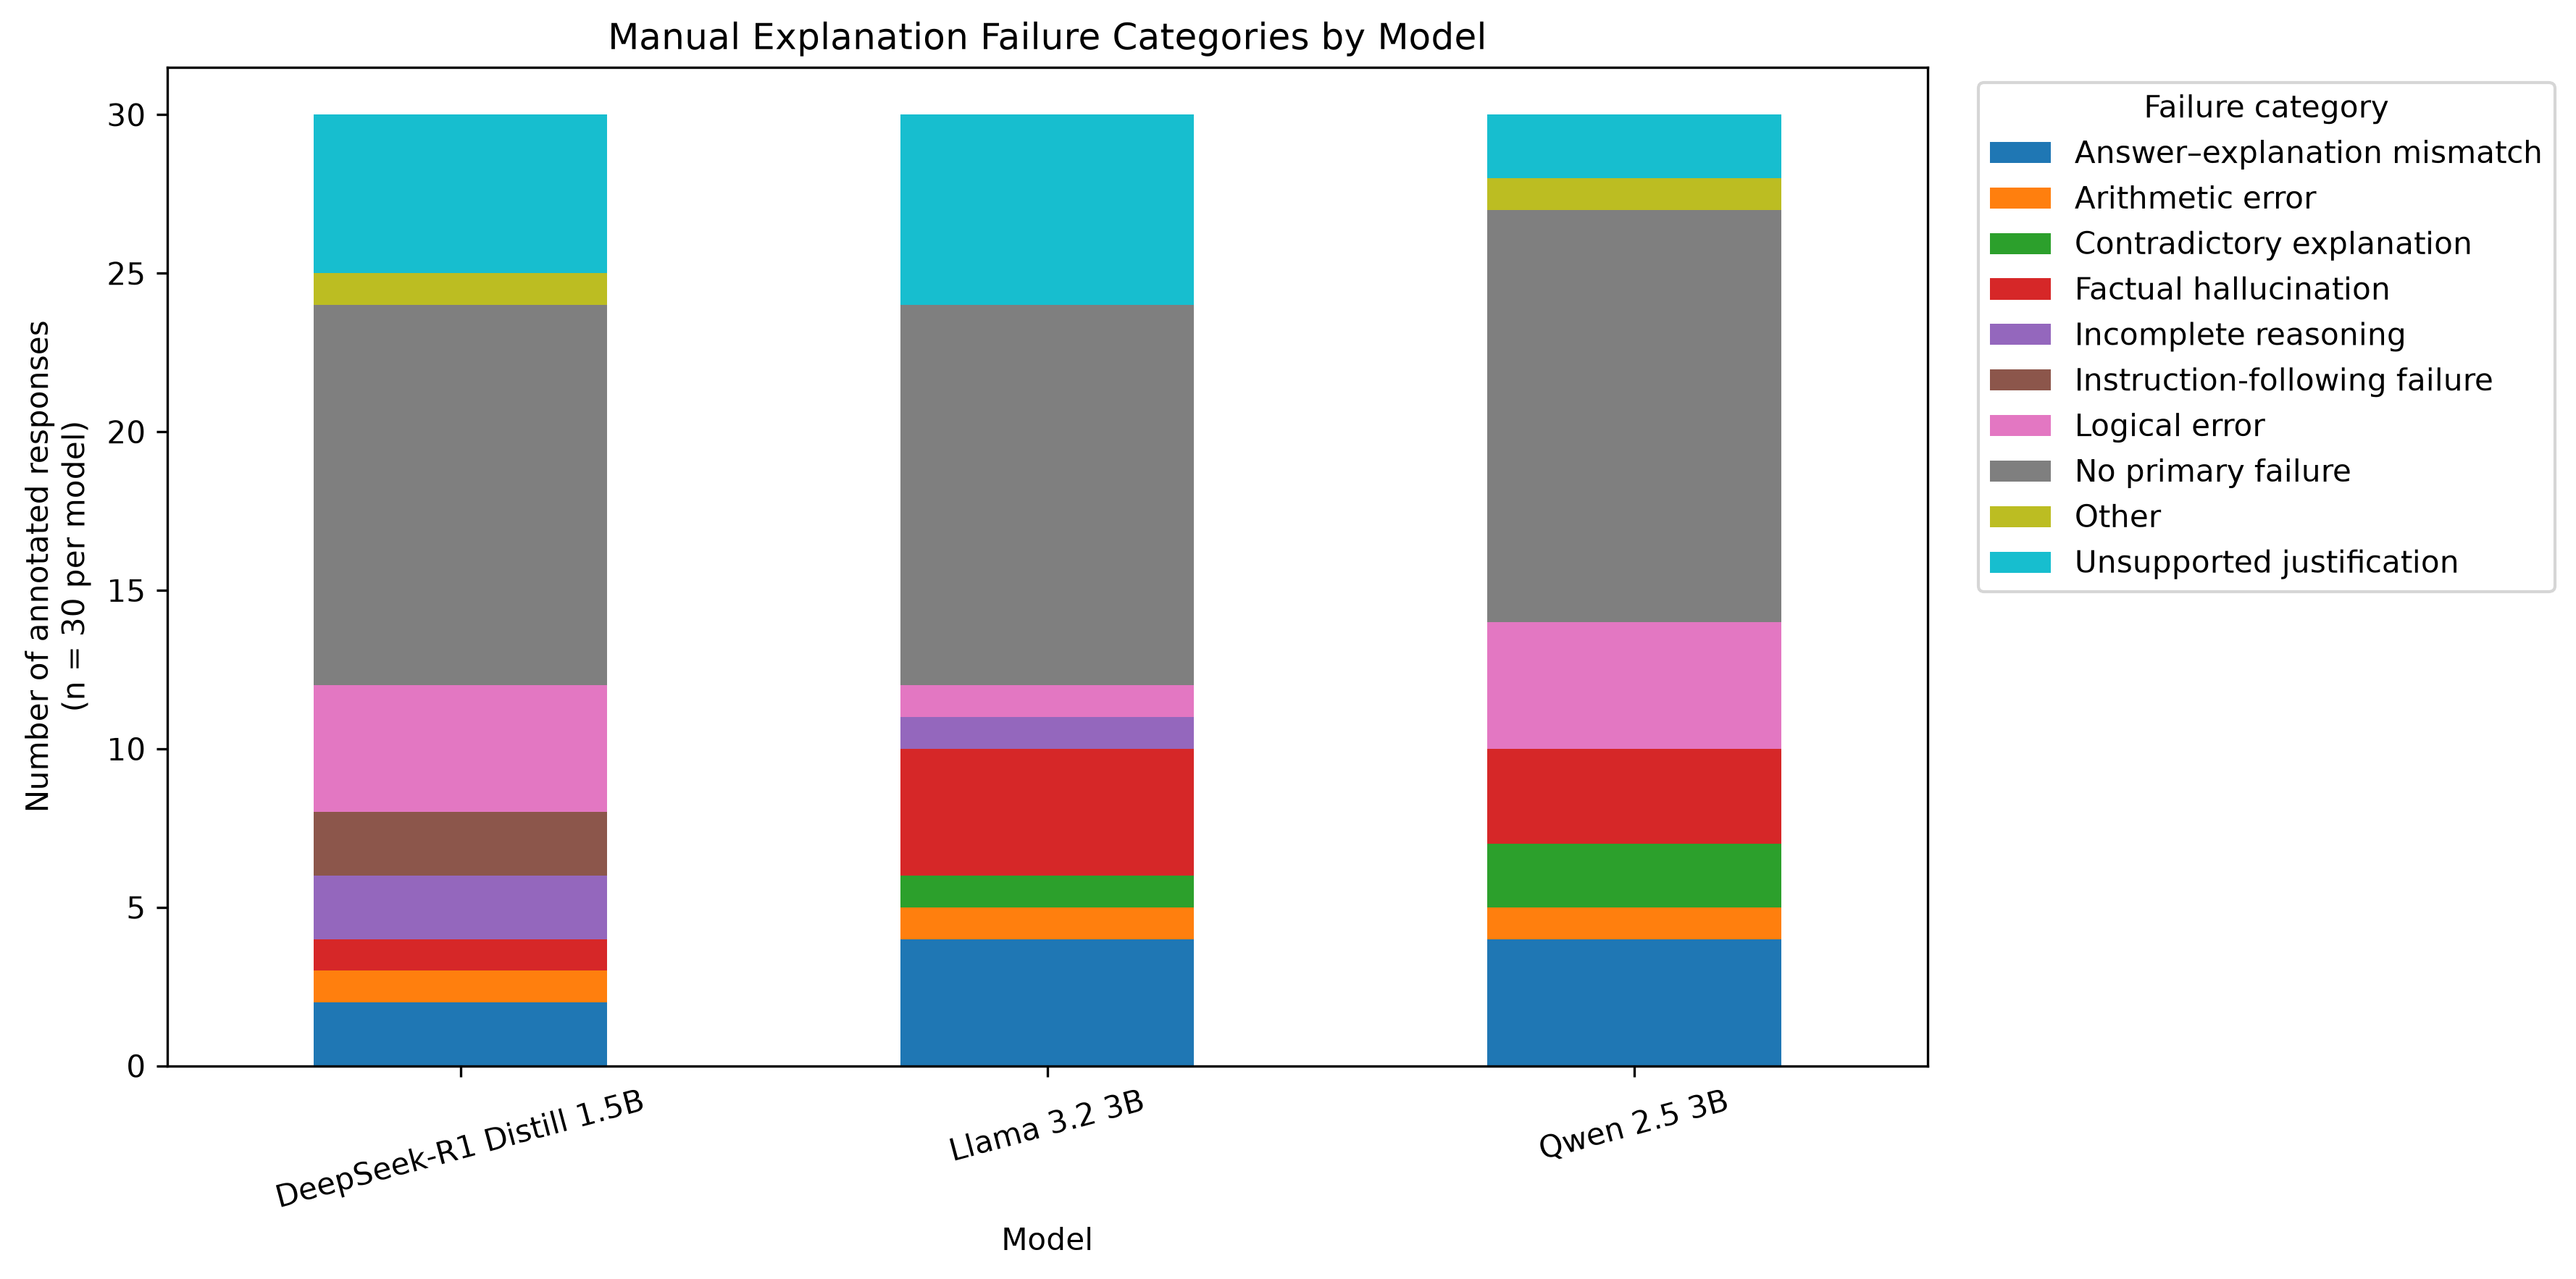
\includegraphics[width=\linewidth]
    {failure_categories_by_model.png}
    \caption{Primary explanation failure categories in the balanced
    manual-analysis sample ($n=30$ per model).}
    \label{fig:failure_categories}
\end{figure}

Unsupported justification was common for DeepSeek and Llama. Llama and
Qwen also exhibited factual hallucinations and answer--explanation
mismatches. Qwen additionally produced contradictory explanations,
particularly on GSM8K, where an explanation sometimes reached one
numerical result while the final answer contained a different value.

Such failures are especially important because the explanation may
appear competent even though the visible reasoning and final prediction
are inconsistent.

\subsection{Qualitative Error Analysis}

To complement the aggregate scores, representative responses were
selected from the reviewed manual-analysis sample. These examples cover
a strong correct explanation, an answer--explanation mismatch, an
unsupported justification, a factual hallucination, and a logical or
arithmetic error.

Table~\ref{tab:qualitative_examples} presents the selected cases.

\begin{table*}[t]
\centering
\small
\caption{Representative qualitative examples from the reviewed manual-analysis sample. Excerpts are shortened for readability.}
\label{tab:qualitative_examples}
\begin{tabular}{llllllp{2.7cm}}
\toprule
\textbf{Model} &
\textbf{Dataset} &
\textbf{Case} &
\textbf{Gold} &
\textbf{Prediction} &
\textbf{Explanation excerpt} &
\textbf{Primary failure} \\
\midrule
DeepSeek-R1 Distill 1.5B & CommonsenseQA & Strong correct explanation & E. tiredness & E & \parbox[t]{4.4cm}{Tiredness is likely because running after a ball would require exerting energy, leading to a sense of fatigue.} & none \\
Llama 3.2 3B & GSM8K & Answer–explanation mismatch & 720 & 960 & \parbox[t]{4.4cm}{Greta first puts 50\% of her paycheck into her retirement account, which is 0.5 * \$2400 = \$1200. Then, she uses 20\% of her paycheck for her car payment, which is 0.2 * \$2400 = \$480…} & answer\_explanation\_mismatch \\
Qwen 2.5 3B & CommonsenseQA & Unsupported justification & D. outside & C. windowsill & \parbox[t]{4.4cm}{Ivy plants often require a lot of sunlight, which they can get from the warm south or west-facing windowsills in homes. Additionally, windowsills provide a stable surface for the…} & unsupported\_justification \\
Llama 3.2 3B & StrategyQA & Factual hallucination & no & B & \parbox[t]{4.4cm}{A modern central processing unit (CPU) circuit chip is typically quite large and bulky, often measuring several inches in size. A house key, on the other hand, is a small, thin ob…} & factual\_hallucination \\
DeepSeek-R1 Distill 1.5B & GSM8K & Logical or arithmetic error & 525 & 580 calories deficit per day & \parbox[t]{4.4cm}{Andy needs to burn 105,000 calories over 181 days, which averages to approximately 580 calories deficit per day.} & logical\_error \\
\bottomrule
\end{tabular}
\end{table*}




\subsection{Statistical Analysis}

Wilson 95\% confidence intervals were calculated for answer accuracy.
Because the manual faithfulness ratings were ordinal scores on a
0--3 scale, explanations accompanying correct and incorrect answers
were compared using a two-sided Mann--Whitney U test. Cliff's delta
was used to quantify the magnitude of the difference, and a
non-parametric bootstrap with 10,000 resamples was used to estimate a
95\% confidence interval for the difference in mean faithfulness
scores.

Across all models, explanations accompanying correct answers obtained
a mean explanation-support faithfulness score of 2.64, compared with
0.89 for explanations accompanying incorrect answers. The mean
difference was 1.76 points, with a bootstrap 95\% confidence interval
of [1.42, 2.07]. The two score distributions differed significantly
($U=1827.0$, $p<0.001$), and Cliff's delta was 0.804, indicating a
large effect.

The same pattern was observed for every model. Qwen showed a mean
difference of 2.00 points
($U=214.0$, $p<0.001$, $\delta=0.902$), while Llama showed a
difference of 1.93 points
($U=211.5$, $p<0.001$, $\delta=0.880$). DeepSeek showed a smaller,
but still large, difference of 1.33 points
($U=183.0$, $p=0.001$, $\delta=0.627$).

These findings provide strong support for H2: explanations associated
with correct answers tend to provide substantially stronger visible
support than explanations associated with incorrect answers. However,
the observed association does not demonstrate that the generated
explanations causally reflect the models' hidden internal reasoning
processes.


\subsection{Results Summary}

The results support all three hypotheses.

First, H1 is supported by the pronounced task-specific performance
differences. DeepSeek-R1 Distill achieved the strongest mathematical
performance on GSM8K, whereas Qwen and Llama were substantially
stronger on CommonsenseQA and StrategyQA. The overlapping overall
confidence intervals indicate that no model can be considered
universally superior on the basis of aggregate accuracy alone.

Second, H2 is strongly supported. Across all models, correct answers
were accompanied by significantly higher explanation-support
faithfulness scores than incorrect answers, with a large overall effect
size. This pattern was also present for each model individually.

Third, the findings support H3. DeepSeek's reasoning-oriented behavior
was associated with substantially stronger GSM8K accuracy, but also
with a larger generation budget, longer inference time, and lower
strict-format success than Qwen and Llama.

Taken together, the results show that no single metric is sufficient
for evaluating these models. DeepSeek achieved the highest observed
overall accuracy and strongest mathematical performance, Llama achieved
the best format compliance and fastest mean generation time, and Qwen
showed the most balanced performance across CommonsenseQA and
StrategyQA. The manual analysis further revealed different strengths
in explanation-support faithfulness, logical consistency, and
completeness.

\section{Discussion}

\subsection{Task Specialization}

The results show that no model is consistently best across all tasks.
This directly addresses RQ1. DeepSeek-R1 Distill is strongly specialized
for mathematical reasoning, whereas Qwen and Llama perform substantially
better on commonsense and strategy questions. The dataset-level
confidence intervals reinforce this pattern, particularly for GSM8K,
where DeepSeek clearly outperforms the other two models.

Task specialization is also visible in explanation quality. DeepSeek's
GSM8K explanations are comparatively strong, while its StrategyQA
explanations receive the lowest mean faithfulness score among the
evaluated model--dataset combinations. This suggests that strong
performance on one reasoning domain does not imply uniformly strong
explanation behavior across other domains.

\subsection{Accuracy and Explanation Quality}

The results for RQ3 show that answer accuracy and explanation quality
are related but distinct. Correct answers usually receive higher
explanation-support faithfulness scores, and this relationship is
statistically strong across all three models. Nevertheless, correct
answers can still be accompanied by incomplete or weak reasoning, while
incorrect answers can be presented with fluent and confident
explanations.

The balanced manual-analysis design makes this distinction especially
visible because the reviewed subset contains equal numbers of correct
and incorrect responses within each model--dataset combination. Without
this balancing step, the manual results could be dominated by easier
correct cases from stronger model--dataset pairs.

Answer--explanation mismatches are particularly concerning. A user may
read a plausible chain of reasoning and fail to notice that the stated
final answer is inconsistent with the explanation. Conversely, a model
may provide a confident but unsupported justification for an incorrect
answer. Explanation fluency should therefore not be treated as a
substitute for answer verification.

\subsection{Instruction Compliance and Efficiency}

The results for RQ2 show that strict output-format compliance was nearly
perfect for Qwen and Llama but substantially lower for DeepSeek.
DeepSeek frequently produced long reasoning traces, repetition,
incomplete generations, or outputs that did not reach both required
fields within the available generation budget.

Increasing the DeepSeek token limit from 256 to 768 improved completion
rates but also increased runtime substantially. This trade-off matters
for practical deployment. A reasoning-oriented model may perform well
on difficult tasks while remaining slower, less predictable, and more
expensive to evaluate.

Because DeepSeek used a larger generation budget than Qwen and Llama,
the runtime comparison should be interpreted as a practical
system-level comparison rather than a perfectly controlled efficiency
benchmark. Even so, the difference reflects an important deployment
cost associated with the model's longer reasoning behavior.

\subsection{Failure Patterns}

The manual failure taxonomy addresses RQ4. Unsupported justification,
factual hallucination, answer--explanation mismatch, contradictory
reasoning, and logical or arithmetic errors occurred across the
evaluated models.

These failures reveal different trust risks. Unsupported justification
creates the appearance of reasoning without sufficient evidence.
Factual hallucination introduces claims that may sound relevant but are
not grounded in the question. Answer--explanation mismatch is especially
problematic because the explanation and final answer may each appear
plausible when inspected separately, even though they are mutually
inconsistent.

The diversity of failure types also shows why a single explanation
metric is insufficient. Faithfulness, logical consistency, completeness,
and failure category capture related but non-identical properties of
the generated explanations.

\subsection{Comparison with Previous Work}

The observed gap between fluent explanation and reliable support is
consistent with previous work showing that chain-of-thought text can be
influenced by irrelevant prompt features and can function as a post-hoc
rationale
\cite{turpin2023language,lanham2023measuring}. The strong difference
between correct and incorrect explanations also aligns with studies
that treat explanation quality as related to, but not identical with,
prediction quality
\cite{madsen2024selfexplanations,paul2024making}.

The results additionally complement broad benchmarking work by showing
why aggregate accuracy alone is insufficient
\cite{liang2023helm}. DeepSeek achieved the highest observed overall
accuracy, yet its strict parse success and runtime were substantially
worse. Conversely, Llama's perfect format compliance did not translate
into strong mathematical accuracy. Trustworthy model selection
therefore requires multiple criteria rather than a single leaderboard
score.

\subsection{Implications for XAI}

The findings support a cautious interpretation of LLM
self-explanations. The manual scores measure whether an explanation
supports the visible answer, not whether it exposes the hidden causal
computation of the neural network. Consequently, these explanations are
best understood as \emph{behavioral justifications}.

Behavioral justifications can still be useful. They allow users,
developers, and evaluators to inspect model outputs and identify
contradictions, hallucinations, incomplete reasoning, and
answer--explanation mismatches. However, they should not be presented as
direct windows into internal model reasoning.

For trustworthy deployment, self-explanations should be combined with
independent answer verification \cite{weng2023selfverification},
uncertainty or hallucination estimation
\cite{manakul2023selfcheckgpt,farquhar2024semantic}, retrieval or tool
support, and explicit consistency checks between the explanation and
the final answer.

\section{Limitations}

This study has several limitations.

First, only three relatively small open-source or open-weight models
were evaluated. The findings may not generalize to larger proprietary
systems, larger open models, or future model families.

Second, the benchmark contains 100 samples per dataset. Although the
same fixed samples were used for every model and confidence intervals
were reported, a larger benchmark would reduce sampling uncertainty and
support stronger model comparisons.

Third, the reviewed manual-analysis sample contains 90 responses. The
sample was balanced across models, datasets, and answer correctness, but
it remains small relative to the full set of 900 generations.

Fourth, the manual evaluation used a single structured review process.
Although the final annotations were reviewed for consistency, the
scores still contain subjective judgment. A stronger evaluation would
use multiple independent annotators and report inter-annotator
agreement.

Fifth, the rubric measures explanation-support faithfulness rather than
causal faithfulness. The study can identify whether the visible
explanation supports the visible answer, but it cannot establish whether
the explanation reflects the hidden computation that produced the
answer.

Sixth, all models were evaluated with 4-bit NF4 quantization on a
consumer GPU with 4\,GB of VRAM. Quantization may affect output quality,
especially on tasks requiring exact numerical reasoning.

Seventh, DeepSeek used a larger maximum generation budget than Qwen and
Llama. This adjustment was necessary to reduce truncation, but it
complicates direct comparison of runtime, output length, and format
compliance.

Eighth, the study uses a single standardized prompt and greedy decoding.
Alternative prompt structures, answer-first versus explanation-first
ordering, few-shot examples, sampling strategies, or self-consistency
could change both accuracy and explanation behavior.

Finally, StrategyQA was evaluated using an available training split from
a Parquet-compatible distribution. Although the same fixed examples were
used for every model, this differs from evaluation on an untouched
official test set and should be considered when interpreting the
results.
\section{Future Work}

Future work should extend the evaluation to larger open-weight and
proprietary models, additional reasoning benchmarks, and multilingual
tasks. A larger benchmark would provide narrower confidence intervals
and support stronger comparisons between model families.

The manual evaluation should also be expanded. Multiple independent
annotators could score the same explanations, enabling the calculation
of inter-annotator agreement and reducing dependence on a single
review process. Future studies could additionally investigate whether
different user groups interpret the same explanation differently.

A particularly important direction is stronger causal evaluation.
Controlled interventions could modify numerical values in GSM8K,
reorder CommonsenseQA options, alter supporting facts in StrategyQA,
remove individual rationale steps, or replace generated explanations
with alternative rationales. The model's answer could then be tested
for appropriate sensitivity to these changes
\cite{lanham2023measuring,matton2025walk,zaman2025causal}.

Future experiments should also compare different prompting and
decoding strategies, including answer-first and explanation-first
prompting, few-shot demonstrations, self-consistency, and constrained
output generation. Such comparisons would help determine whether the
observed failure patterns are properties of the models or consequences
of the selected generation protocol.

Finally, automated detectors for answer--explanation mismatch,
unsupported justification, factual hallucination, and contradictory
reasoning could make explanation analysis more scalable. These systems
could combine semantic consistency checks, numerical verification,
retrieval-based fact checking, and uncertainty estimation.

\section{Conclusion}

This paper presented a controlled empirical evaluation of
self-generated explanations from Qwen~2.5~3B, Llama~3.2~3B, and
DeepSeek-R1 Distill Qwen~1.5B on GSM8K, CommonsenseQA, and
StrategyQA. The evaluation covered 900 generated responses and combined
answer accuracy, strict output-format compliance, runtime measurement,
manual explanation scoring, failure-category analysis, and statistical
testing.

The models exhibited clear task specialization. DeepSeek-R1 Distill
achieved the strongest mathematical performance on GSM8K, whereas
Qwen performed best on CommonsenseQA and StrategyQA. Llama achieved
perfect strict-format compliance and the fastest mean generation time.
These differences show that aggregate accuracy alone is insufficient
for comparing model reliability.

The reviewed analysis of 90 balanced responses showed that explanations
accompanying correct answers received substantially higher
explanation-support faithfulness scores than explanations accompanying
incorrect answers. The difference was statistically significant and
corresponded to a large effect. Nevertheless, all three models produced
observable failures, including unsupported justifications, factual
hallucinations, arithmetic and logical errors, contradictory
explanations, and answer--explanation mismatches.

The findings demonstrate that natural-language self-explanations can
provide useful behavioral evidence about model outputs, but they should
not be interpreted as direct proof of faithful internal reasoning.
Reliable use of LLM explanations therefore requires independent answer
verification, consistency checking, uncertainty estimation, and careful
attention to task-specific failure patterns.

\appendix

\section{Standardized Prompt}
\label{app:prompt}

All models received the same output-format instruction:

\begin{quote}
\texttt{FINAL\_ANSWER: <answer>}\\
\texttt{EXPLANATION: <concise justification>}
\end{quote}

The task-specific instructions differed only in the expected answer
format.

\begin{itemize}
    \item \textbf{GSM8K}: the model was instructed to return a numerical
    answer.

    \item \textbf{CommonsenseQA}: the model was instructed to return the
    selected option label, with option text permitted as additional
    content.

    \item \textbf{StrategyQA}: the model was instructed to return a
    binary yes/no answer.
\end{itemize}

The final answer was requested before the explanation. This ordering
made the prediction easier to extract and allowed the same strict parser
to be applied across all models.

\section{Manual Annotation Procedure}
\label{app:annotation}

The reviewed manual-analysis sample contained 90 successfully parsed
responses. Ten responses were selected from each model--dataset
combination, with five correct and five incorrect answers whenever
possible.

This produced the following balanced design:

\[
3\ \text{models}
\times
3\ \text{datasets}
\times
10\ \text{responses}
=
90\ \text{reviewed responses}.
\]

Each response was assessed on three dimensions:

\begin{itemize}
    \item \textbf{Explanation-support faithfulness}: whether the
    explanation correctly supports the model's stated final answer;

    \item \textbf{Logical consistency}: whether the reasoning is
    coherent and free from internal contradiction;

    \item \textbf{Completeness}: whether the explanation contains
    sufficient reasoning to justify the stated answer.
\end{itemize}

Each dimension was assigned a score from 0 to 3.

\begin{table}[h]
\centering
\caption{Detailed interpretation of the manual explanation scores.}
\label{tab:appendix_rubric}
\begin{tabular}{cp{10.5cm}}
\toprule
\textbf{Score} & \textbf{Interpretation} \\
\midrule
0 &
The explanation is absent, unrelated, contradictory, or provides no
meaningful support for the final answer. \\

1 &
The explanation contains major factual, logical, or arithmetic errors,
or provides only weak support. \\

2 &
The explanation provides partial support but includes missing,
unsupported, incomplete, or flawed reasoning. \\

3 &
The explanation provides clear, correct, logically consistent, and
sufficient support for the final answer. \\
\bottomrule
\end{tabular}
\end{table}

A primary failure category was additionally assigned to every reviewed
response. The taxonomy contained:

\begin{itemize}
    \item \textbf{Answer--explanation mismatch}: the explanation supports
    a conclusion different from the stated final answer;

    \item \textbf{Arithmetic error}: the explanation contains an
    incorrect numerical operation or calculation;

    \item \textbf{Contradictory explanation}: different parts of the
    explanation are mutually inconsistent;

    \item \textbf{Factual hallucination}: the explanation introduces
    unsupported or false factual claims;

    \item \textbf{Incomplete reasoning}: necessary steps are missing;

    \item \textbf{Instruction-following failure}: the required answer or
    explanation format is not followed;

    \item \textbf{Logical error}: the conclusion does not follow from
    the stated premises;

    \item \textbf{Unsupported justification}: the explanation asserts a
    conclusion without sufficient evidence;

    \item \textbf{Other}: the failure does not fit the predefined
    categories;

    \item \textbf{No primary failure}: no major explanation failure was
    identified.
\end{itemize}

The annotation procedure evaluates visible behavioral support. It does
not establish that the generated explanation is causally identical to
the hidden internal computation that produced the answer.

\section{Additional Accuracy Results}
\label{app:accuracy}

Table~\ref{tab:appendix_accuracy} reports the complete Wilson 95\%
confidence intervals for all model--dataset combinations.

\begin{table*}[t]
\centering
\small
\caption{Answer accuracy with Wilson 95\% confidence intervals.}
\label{tab:appendix_accuracy}
\begin{tabular}{llrrr}
\toprule
\textbf{Model} &
\textbf{Dataset} &
\textbf{Correct} &
\textbf{Accuracy (\%)} &
\textbf{95\% CI} \\
\midrule
Qwen 2.5 3B & GSM8K & 13/100 & 13.00 & [7.76, 20.98] \\
Qwen 2.5 3B & CommonsenseQA & 76/100 & 76.00 & [66.77, 83.31] \\
Qwen 2.5 3B & StrategyQA & 60/100 & 60.00 & [50.20, 69.06] \\
Qwen 2.5 3B & Overall & 149/300 & 49.67 & [44.05, 55.29] \\
\midrule
Llama 3.2 3B & GSM8K & 6/100 & 6.00 & [2.78, 12.48] \\
Llama 3.2 3B & CommonsenseQA & 70/100 & 70.00 & [60.42, 78.11] \\
Llama 3.2 3B & StrategyQA & 59/100 & 59.00 & [49.20, 68.13] \\
Llama 3.2 3B & Overall & 135/300 & 45.00 & [39.47, 50.66] \\
\midrule
DeepSeek-R1 Distill 1.5B & GSM8K & 80/100 & 80.00 & [71.12, 86.66] \\
DeepSeek-R1 Distill 1.5B & CommonsenseQA & 28/100 & 28.00 & [20.14, 37.49] \\
DeepSeek-R1 Distill 1.5B & StrategyQA & 49/100 & 49.00 & [39.42, 58.65] \\
DeepSeek-R1 Distill 1.5B & Overall & 157/300 & 52.33 & [46.69, 57.92] \\
\bottomrule
\end{tabular}
\end{table*}

The overall confidence intervals overlap substantially. Therefore, the
aggregate accuracy differences should not be interpreted as decisive
evidence that one model is universally superior.

\section{Additional Faithfulness Statistics}
\label{app:statistics}

Table~\ref{tab:appendix_statistics} reports the correct-versus-incorrect
faithfulness comparisons.

\begin{table*}[t]
\centering
\small
\caption{Faithfulness comparison between correct and incorrect
responses.}
\label{tab:appendix_statistics}
\begin{tabular}{lrrrrrr}
\toprule
\textbf{Scope} &
\textbf{Correct mean} &
\textbf{Incorrect mean} &
\textbf{Difference} &
\textbf{Bootstrap 95\% CI} &
\textbf{$p$-value} &
\textbf{Cliff's $\delta$} \\
\midrule
All models &
2.64 &
0.89 &
1.76 &
[1.42, 2.07] &
$<0.001$ &
0.804 \\

Qwen 2.5 3B &
2.73 &
0.73 &
2.00 &
[1.47, 2.47] &
$<0.001$ &
0.902 \\

Llama 3.2 3B &
2.67 &
0.73 &
1.93 &
[1.40, 2.40] &
$<0.001$ &
0.880 \\

DeepSeek-R1 Distill 1.5B &
2.53 &
1.20 &
1.33 &
[0.67, 1.93] &
0.001 &
0.627 \\
\bottomrule
\end{tabular}
\end{table*}

All observed Cliff's delta values correspond to large effects. Positive
values indicate that explanations attached to correct answers generally
received higher explanation-support faithfulness scores than
explanations attached to incorrect answers.

\section{Qualitative Examples}
\label{app:qualitative}

The complete set of selected representative examples is included in
Table~\ref{tab:qualitative_examples}. These examples cover:

\begin{itemize}
    \item a strong correct explanation;
    \item an answer--explanation mismatch;
    \item an unsupported justification;
    \item a factual hallucination;
    \item a logical or arithmetic error.
\end{itemize}

\begin{table*}[t]
\centering
\small
\caption{Representative qualitative examples from the reviewed manual-analysis sample. Excerpts are shortened for readability.}
\label{tab:qualitative_examples}
\begin{tabular}{llllllp{2.7cm}}
\toprule
\textbf{Model} &
\textbf{Dataset} &
\textbf{Case} &
\textbf{Gold} &
\textbf{Prediction} &
\textbf{Explanation excerpt} &
\textbf{Primary failure} \\
\midrule
DeepSeek-R1 Distill 1.5B & CommonsenseQA & Strong correct explanation & E. tiredness & E & \parbox[t]{4.4cm}{Tiredness is likely because running after a ball would require exerting energy, leading to a sense of fatigue.} & none \\
Llama 3.2 3B & GSM8K & Answer–explanation mismatch & 720 & 960 & \parbox[t]{4.4cm}{Greta first puts 50\% of her paycheck into her retirement account, which is 0.5 * \$2400 = \$1200. Then, she uses 20\% of her paycheck for her car payment, which is 0.2 * \$2400 = \$480…} & answer\_explanation\_mismatch \\
Qwen 2.5 3B & CommonsenseQA & Unsupported justification & D. outside & C. windowsill & \parbox[t]{4.4cm}{Ivy plants often require a lot of sunlight, which they can get from the warm south or west-facing windowsills in homes. Additionally, windowsills provide a stable surface for the…} & unsupported\_justification \\
Llama 3.2 3B & StrategyQA & Factual hallucination & no & B & \parbox[t]{4.4cm}{A modern central processing unit (CPU) circuit chip is typically quite large and bulky, often measuring several inches in size. A house key, on the other hand, is a small, thin ob…} & factual\_hallucination \\
DeepSeek-R1 Distill 1.5B & GSM8K & Logical or arithmetic error & 525 & 580 calories deficit per day & \parbox[t]{4.4cm}{Andy needs to burn 105,000 calories over 181 days, which averages to approximately 580 calories deficit per day.} & logical\_error \\
\bottomrule
\end{tabular}
\end{table*}


\section{Reproducibility Details}
\label{app:reproducibility}

The final processed benchmark contained 300 questions and used random
seed 42. It was stored in CSV and JSONL formats.

The SHA-256 checksum of the final processed benchmark CSV was:

\begin{quote}
\small
\texttt{35b721529e523d4a945407053ded18d93489e5476a23ec90fad1923fb36906e5}
\end{quote}

The complete experiment generated 900 responses:

\[
3\ \text{models}
\times
3\ \text{datasets}
\times
100\ \text{samples}
=
900\ \text{responses}.
\]

Qwen and Llama used a maximum generation budget of 256 new tokens.
DeepSeek used 768 new tokens because shorter generations frequently
ended before both required output fields were completed.

All three models were loaded using:

\begin{itemize}
    \item 4-bit NF4 quantization;
    \item double quantization;
    \item float16 computation;
    \item greedy deterministic decoding;
    \item random seed 42.
\end{itemize}

The experiments were conducted using:

\begin{itemize}
    \item Windows;
    \item Python~3.11.2;
    \item PyTorch~2.7.1;
    \item CUDA~11.8;
    \item NVIDIA GeForce GTX~1650~Ti;
    \item 4\,GB VRAM.
\end{itemize}

The stored result files preserve the model identifier, dataset,
sample identifier, prompt, raw generation, parsed answer, extracted
explanation, ground truth, correctness label, generation time, parse
status, and error field.

\section{Reproduction Commands}
\label{app:commands}

The primary evaluation stages were:

\begin{verbatim}
python -m src.prepare_data
python -m src.inspect_data
python -m src.run_inference
python -m src.evaluate_answers
python -m src.combine_results
python -m src.select_balanced_annotations
python -m src.analyze_manual_annotations
python -m src.statistical_analysis
python -m src.select_qualitative_examples
python -m src.create_paper_figures
\end{verbatim}

The exact model, dataset, input, and output arguments are preserved in
the repository configuration and experiment files.



\bibliographystyle{plain}
\bibliography{references}

\end{document}


